%! suppress = GroupedSubSupScript
%! suppress = Ellipsis
% Define document class
\documentclass[twocolumn,twocolappendix,linenumbers]{aastex631}
%\documentclass[twocolumn,twocolappendix]{aastex631}
%\documentclass[modern,linenumbers]{aastex631}

% Some entries inspired from a preamble by Adrian Price-Whelan, https://github.com/adrn/PhaseSpiralAsteroseismology/blob/main/tex/preamble.tex

\usepackage{showyourwork}

% Latex imports
\let\tablenum\relax             % necessary for AASTeX
\usepackage{siunitx}
\sisetup{range-phrase= \text{--}, range-units=single, separate-uncertainty=true}
\sisetup{separate-uncertainty=true}
\usepackage{blindtext}          % Filler text
\usepackage{xcolor}
\usepackage[T1]{fontenc}

\usepackage[toc,nogroupskip,nohypertypes={glossary}]{glossaries} % import after hyperref
\glsdisablehyper

\newglossaryentry{HST}{name={HST}, description={Hubble Space Telescope}, first={Hubble Space Telescope (HST)}}
\newglossaryentry{NIR}{name={NIR}, description={Near-Infrared}, first={near-infrared (NIR)}}
\newglossaryentry{MIR}{name={MIR}, description={Mid-Infrared}, first={mid-infrared (MIR)}}
\newglossaryentry{FIR}{name={FIR}, description={Far-Infrared}, first={far-infrared (FIR)}}
\newglossaryentry{FUV}{name={FUV}, description={Far-Ultraviolet}, first={far-Ultraviolet (FUV)}}
\newglossaryentry{NUV}{name={NUV}, description={Near-Ultraviolet}, first={near-Ultraviolet (NUV)}}
\newglossaryentry{EUV}{name={EUV}, description={extreme-Ultraviolet}, first={extreme-Ultraviolet (EUV)}}
\newglossaryentry{SED}{name={SED}, description={Spectral energy distribution}, first={spectral energy distribution (SED)}, firstplural={spectral energy distributions (SEDs)}}
\newglossaryentry{ppm}{name={ppm}, description={parts per million}, first={parts per million (ppm)}}
\newglossaryentry{PDF}{name={PDF}, description={Probability density function}, first={probability density function (PDF)}, firstplural={probability density functions (PDF)}}
\newglossaryentry{PLATO}{name={PLATO}, description={PLAnetary Transits and Oscillations of stars}, first={PLATO~\citep[][]{Rauer2014}}}
\newglossaryentry{PSF}{name={PSF},description={Point Spread Function}, first={point spread function (PSF)}, firstplural={point spread functions (PSF)}}
\newglossaryentry{SFD}{name={SFD}, description={Size frequency distribution}, first={size frequency distribution (SFD)}, firstplural={Size frequency distributions (SFD)}}
\newglossaryentry{SNR}{name={SNR}, description={Signal-to-noise ratio}, first={signal-to-noise ratio (SNR)}}
\newglossaryentry{RV}{name={RV}, description={Radial Velocity}, first={Radial Velocity (RV)}, firstplural={Radial Velocities (RV)}}
\newglossaryentry{TTV}{name={TTV}, description={Transit Timing Variation}, first={transit timing variation (TTV)}, firstplural={transit timing variations (TTVs)}}
\newglossaryentry{TESS}{name={TESS}, description={Transiting Exoplanet Survey Satellite}, first={Transiting Exoplanet Survey Satellite~\citep[\textit{TESS},][]{Ricker2014}}}
\newglossaryentry{TIC}{name={TIC}, description={\textit{TESS} Input Catalog}, first={\textit{TESS} Input Catalog~\citep[TIC,][]{Stassun2018}}}
\newglossaryentry{JWST}{name={JWST}, description={James Webb Space Telescope}, first={James Webb Space Telescope~\citep[\textit{JWST},][]{Beichman2014}}}
\newglossaryentry{HZ}{name={HZ}, description={habitable zone}, first={habitable zone (HZ)}}
\newglossaryentry{EEC}{name={EEC}, description={exo-Earth candidate}, first={exo-Earth candidate (EEC)}, firstplural={exo-Earth candidates (EEC)}}
%\newglossaryentry{}{name={}, description={}, first={}, firstplural={}}


% package to open file containing variables
\usepackage{datatool, filecontents}
\DTLsetseparator{,}% Set the separator between the columns.

% import data
\DTLloaddb[noheader, keys={thekey,thevalue}]{variables}{variables.dat}
% Loads variables.dat with column headers 'thekey' and 'thevalue'
\newcommand{\var}[1]{\ensuremath{\DTLfetch{variables}{thekey}{#1}{thevalue}}}

% paper comments
\usepackage{comment}						 % comments that can be switched visible/invisible
\includecomment{comment}
%\specialcomment{outtake}{\begingroup\sffamily\color{gray}}{\endgroup}
%\specialcomment{note}{\begingroup\sffamily\color{red!40!green!70!blue!90}}{\endgroup}
\specialcomment{note}{\begingroup\sffamily\color{gray}}{\endgroup}
%\excludecomment{note}                       % switch notes off

%% switch TODO notes on/off
\usepackage[backgroundcolor=red!20!green!40!blue!10, textsize=tiny]{todonotes}
% \usepackage[disable]{todonotes}			% switches all todo notes to invisible
\usepackage{regexpatch}
\makeatletter
\xpatchcmd{\@todo}{\setkeys{todonotes}{#1}}{\setkeys{todonotes}{inline,#1}}{}{}
\makeatother

%% manuscript revision
%\newcommand{\rev}[1]{{\textbf{#1}}}    % on
\newcommand{\rev}[1]{{#1}}              % off

%% ... and second revision
\newcommand{\revv}[1]{{\textbf{#1}}}    % on
%\newcommand{\revv}[1]{{#1}}            % off

% ---------------------------------
% PAPER VARIABLES

% ---------------------------------
% CONSTANTS/MISSIONS/ABBREVIATIONS

% SIunitx definitions
\DeclareSIUnit\mSun{M_\odot}
\DeclareSIUnit\Msun{M_\odot}
\DeclareSIUnit\mStar{M_\star}
\DeclareSIUnit\Mstar{M_\star}
\DeclareSIUnit\mEarth{M_\oplus}
\DeclareSIUnit\Mearth{M_\oplus}
\DeclareSIUnit\rEarth{R_\oplus}
\DeclareSIUnit\Rearth{R_\oplus}
\DeclareSIUnit\year{yr}
\DeclareSIUnit\au{au}
\DeclareSIUnit\dex{dex}
\DeclareSIUnit\ppm{ppm}
\DeclareSIUnit\eV{eV}
\DeclareSIUnit\parsec{pc}
\DeclareSIUnit\photons{photons}
\DeclareSIUnit\erg{erg}

% Missions/Projects/Packages
\newcommand{\code}[1]{\texttt{#1}}
\newcommand{\project}[1]{\textsl{#1}}

\newcommand{\bioverse}{\code{Bioverse}}
\newcommand{\emcee}{\project{emcee}}

\newcommand{\rst}{\project{Nancy Grace Roman Space Telescope}}
\newcommand{\plato}{\project{PLATO}}
\newcommand{\cheops}{\project{CHEOPS}}
\newcommand{\kepler}{\project{Kepler}}
\newcommand{\ktwo}{\project{K2}}
\newcommand{\tess}{\project{TESS}}
\newcommand{\ariel}{\project{Ariel}}
\newcommand{\nautilus}{\project{Nautilus}}
\newcommand{\life}{\project{LIFE}}
\newcommand{\hwo}{\project{Habitable Worlds Observatory}}
\newcommand{\gclef}{\project{G-CLEF}}
\newcommand{\gmt}{\project{Giant Magellan Telescope}}
\newcommand{\andes}{\project{ANDES}}
\newcommand{\elt}{\project{European Extremely Large Telescope}}
\newcommand{\modhis}{\project{MODHIS}}
\newcommand{\tmt}{\project{Thirty Meter Telescope}}
\newcommand{\gaia}{\project{Gaia}}

% Stats / probability
\newcommand{\given}{\,|\,}
\newcommand{\norm}{\mathcal{N}}
\newcommand{\pdf}{\textsl{P}}
%\newcommand{\GG}{\mathbb{G}}
%\newcommand{\pbio}{\mathrm{}}

% Maths
\newcommand{\dd}{\mathrm{d}}
\newcommand{\transpose}[1]{{#1}^{\mathsf{T}}}
\newcommand{\inverse}[1]{{#1}^{-1}}
\newcommand{\argmin}{\operatornamewithlimits{argmin}}
\newcommand{\mean}[1]{\left< #1 \right>}

% Non-scalar variables
\renewcommand{\vec}[1]{\ensuremath{\bs{#1}}}
\newcommand{\mat}[1]{\ensuremath{\mathbf{#1}}}

% Unit shortcuts
\newcommand{\msun}{\ensuremath{\mathrm{M}_\odot}}
\newcommand{\mjup}{\ensuremath{\mathrm{M}_{\mathrm{J}}}}
\newcommand{\kms}{\ensuremath{\mathrm{km}~\mathrm{s}^{-1}}}
\newcommand{\mps}{\ensuremath{\mathrm{m}~\mathrm{s}^{-1}}}
\newcommand{\pc}{\ensuremath{\mathrm{pc}}}
\newcommand{\kpc}{\ensuremath{\mathrm{kpc}}}
\newcommand{\kmskpc}{\ensuremath{\mathrm{km}~\mathrm{s}^{-1}~\mathrm{kpc}^{-1}}}
\newcommand{\dayd}{\ensuremath{\mathrm{d}}}
\newcommand{\yr}{\ensuremath{\mathrm{yr}}}
\newcommand{\AU}{\ensuremath{\mathrm{AU}}}
\newcommand{\Kel}{\ensuremath{\mathrm{K}}}

% Misc.
\newcommand{\bs}[1]{\boldsymbol{#1}}

% Astronomy
\newcommand{\feh}{\ensuremath{{[{\rm Fe}/{\rm H}]}}}
\newcommand{\mh}{\ensuremath{{[{\rm M}/{\rm H}]}}}
\newcommand{\logg}{\ensuremath{\log g}}
\newcommand{\Teff}{\ensuremath{T_{\textrm{eff}}}}
\newcommand{\vsini}{\ensuremath{v\,\sin i}}
%! suppress = LineBreak
\begin{document}

% Title
%\title{Bioverse: Exoplanet Biosignature Detection Under the UV Threshold Hypothesis}
%\title{Bioverse: Exoplanet Biosignature Patterns Under the UV Threshold Hypothesis for the Origin of Life}
\title{Bioverse: Potentially Observable Exoplanet Biosignature Patterns Under the UV Threshold Hypothesis for the Origin of Life}
% The Role of Ultraviolet Radiation in Abiogenesis: Insights from Exoplanet Survey Simulations
% Bioverse: The Impact of UV Flux on Exoplanet Biosignatures under the Cyanosulfidic Origins of Life Scenario

% Author list
\author[0000-0001-8355-2107]{Martin Schlecker}
%\author[0000-0001-8355-2107]{Martin Schlecker} # issue with ORCID? https://github.com/showyourwork/showyourwork/issues/454
\affiliation{Steward Observatory, The University of Arizona, Tucson, AZ 85721, USA; \href{mailto:schlecker@arizona.edu}{schlecker@arizona.edu}}
\author[0000-0003-3714-5855]{D\'{a}niel Apai}
\affiliation{Steward Observatory, The University of Arizona, Tucson, AZ 85721, USA; \href{mailto:schlecker@arizona.edu}{schlecker@arizona.edu}}
\affiliation{Lunar and Planetary Laboratory, The University of Arizona, Tucson, AZ 85721, USA}
\author[0000-0003-3481-0952]{Antonin Affholder}
\affiliation{Department of Ecology and Evolutionary Biology, University of Arizona, Tucson AZ, USA}
\author[0000-0002-5147-9053]{Sukrit Ranjan}
\affiliation{Lunar and Planetary Laboratory, The University of Arizona, Tucson, AZ 85721, USA}
\affiliation{Blue Marble Space Institute of Science, Seattle, 98104, USA}
\author[0000-0002-5806-5566]{Régis Ferrière}
\affiliation{Department of Ecology and Evolutionary Biology, University of Arizona, Tucson AZ, USA}
\affiliation{Institut de Biologie de l'École Normale Supérieure, ENS, PSL, Paris, France}
\affiliation{International Research Laboratory for Interdisciplinary Global Environmental Studies (iGLOBES), CNRS, ENS, PSL, University of Arizona, Tucson AZ, USA}
\author[0000-0003-3702-0382]{Kevin K.\ Hardegree-Ullman}
\affiliation{Steward Observatory, The University of Arizona, Tucson, AZ 85721, USA; \href{mailto:schlecker@arizona.edu}{schlecker@arizona.edu}}
\author[0000-0002-3286-7683]{Tim Lichtenberg}
\affiliation{Kapteyn Astronomical Institute, University of Groningen, PO Box 800, 9700 AV Groningen, The Netherlands}
\author[0000-0003-3557-6256]{Stéphane Mazevet}
\affiliation{Observatoire de la Côte d'Azur, Université Côte d'Azur, Nice, France}






\begin{abstract}
A wide variety of scenarios for the origin of life have been proposed, with many influencing the prevalence and distribution of biosignatures across exoplanet populations.
This relationship suggests these scenarios can be tested by predicting biosignature distributions and comparing them with empirical data.
Here, we demonstrate this approach by focusing on the cyanosulfidic origins-of-life scenario and investigating the hypothesis that a minimum near-ultraviolet (NUV) flux is necessary for abiogenesis.
Using Bayesian modeling and the \bioverse\ survey simulator, we constrain the probability of obtaining strong evidence for or against this ``UV Threshold Hypothesis'' with future biosignature surveys.
Our results indicate that a correlation between past NUV flux and current biosignature occurrence is testable for sample sizes of $\gtrsim$50 planets.
The diagnostic power of such tests is critically sensitive to the intrinsic abiogenesis rate and host star properties, particularly maximum past NUV fluxes.
Surveys targeting a wide range of fluxes, and planets orbiting M dwarfs enhance the chances of conclusive results, with sample sizes $\gtrsim$100 providing $\gtrsim$80\% likelihood of strong evidence if abiogenesis rates are high and the required NUV fluxes are moderate.
For required fluxes exceeding a few hundred erg/s/cm$^2$, both the fraction of inhabited planets and the diagnostic power sharply decrease.
Our findings demonstrate the potential of exoplanet surveys to test origins-of-life hypotheses.
 Beyond specific scenarios, this work underscores the broader value of realistic survey simulations for future observatories (e.g., HWO, LIFE, ELTs, Nautilus) in identifying testable science questions, optimizing mission strategies, and advancing theoretical and experimental studies of abiogenesis.
% This approach emphasizes the need to contextualize biosignature detections, enhancing their credibility and offering new approaches to explore the emergence of life on Earth and beyond.
\end{abstract}

\section{Introduction}
\label{sec:intro}
A wide variety of scenarios for the origin of life have been proposed~\citep[e.g.,][]{Baross1985,Brasier2011,Mulkidjanian2012,Fox2013,Deamer2015,Westall2018}.
While we may still be far from conclusively testing these scenarios, new prospects in the search for conditions favorable to life have opened up by thinking of the origin of life as a planetary phenomenon and identifying global-scale environmental properties that might support pathways to life~\citep{Sasselov2020}.
In particular, specific planetary conditions are needed to create stockpiles of initial compounds for prebiotic chemistry; and planetary processes are required to trigger the prebiotic synthesis.
Such planetary conditions can be hypothesized for exoplanets located in the \gls{HZ} of their host star, with persistent liquid water on their surface.
For example, if deep-sea or sedimentary hydrothermalism is required for abiogenesis, then the insulation of an ocean from the planetary crust minerals (e.g., due to high-pressure ices) may reduce or eliminate the chances of life emerging~\citep[e.g.,][]{Baross1985}.
The alternate scenario of a surface locally subject to wet-dry cycles requires a planetary exposure to mid-range \gls{UV} irradiation, as a source of energy and an agent of selection in chemical evolution~\citep[e.g.,][]{Deamer2019}.
This “UV Threshold Hypothesis” states that \gls{UV} light in a specific wavelength range played a constructive role in getting life started on Earth~\citep{Ranjan2016,Ranjan2017c,Rimmer2018,Rapf2016}, and it could provide a probabilistic approach to the interpretation of possible future biosignature detections~\citep[e.g.,][]{Catling2018,Walker2018}.

The association of chemical pathways to life and planetary environmental conditions offers a new opportunity to test alternate scenarios for life emergence based on planetary-level data collected from the upcoming observations of populations of exoplanets.
Deep-sea hydrothermal scenarios require planetary conditions that may not be met on ocean worlds with large amounts of water, where the water pressure on the ocean floor is high enough to form high-pressure ices~\citep{Noack2016,Kite2018}.  % TODO Sleep et al., 2011? Sobotta et al., 2020?
%\todo[inline]{see discussion in Kite \& Ford 2018 Sect. 6.4}
In this case, a testable prediction would be that planets with high-pressure ices do not show biosignatures.
Likewise, if \gls{UV} light is required to get life started, then there is a minimum planetary \gls{UV} flux requirement to have an inhabited world.
This requirement is set by competing thermal processes; if the photoreaction does not move forward at a rate faster than the competitor thermal process(es), then the abiogenesis scenario cannot function.
On the other hand, abundant \gls{UV} light vastly in excess of this threshold does not increase the probability of abiogenesis, since once the \gls{UV} photochemistry is no longer limiting, some other thermal process in the reaction network will be the rate-limiting process instead.
Therefore, a putative dependence of life on \gls{UV} light is best described as a step function~\citep[e.g.,][]{Ranjan2017c,Rimmer2018,Rimmer2021}.

The goal of this work is to evaluate the potential of future exoplanet surveys to test the hypothesis that a minimum past NUV flux is required for abiogenesis.
We focus on one version of the UV Threshold Hypothesis, the so-called cyanosulfidic scenario, which has been refined to the point where the required threshold flux has been measured to be $F_\mathrm{NUV, min} = \SI{6.8\pm3.6 e10}{\photons\per\centi\meter\squared\per\second\per\nano\meter}$ integrated from \SIrange{200}{280}{\nano\meter} at the surface~\citep{Rimmer2018,Rimmer2021a,Rimmer2023,Ranjan2023a}.
%\todo[inline]{SR: This is an interesting number, because it is below what was available on early Earth (so this scenario could have worked on early Earth) but until recently it was below what was thought to be available on \gls{HZ} M-dwarf exoplanets. So it was thought that identification of biosignatures on M-dwarf planets could therefore falsify the cyanosulfidic scenario, with a potential caveat for transient UV from flares. Two recent developments have complicated the picture. First, Rimmer et al. 2018 had an error in their radiative transfer routines. Correcting for this error, early M-dwarfs and highly active M-dwarfs emit enough UV to meet the Rimmer et al. 2018 criterion (Ranjan et al. 2023).
%\sout{Second, a recent publication argues that /all/ estimates of M-dwarf UV are underestimates, and that late M-dwarf stars have similar emission to Sunlike stars (Rekhi et al. 2023). I suspect this is incorrect, because it contradicts a lot of work from e.g. the MUSCLES collaboration and the HAZMAT project, but it's worth keeping an eye on in case it is correct after all.}}

We follow a semi-analytical Bayesian analysis to estimate probabilities of obtaining strong evidence for or against this hypothesis.
Under the UV Threshold Hypothesis ($H_1$), the probability of an exoplanet having detectable biosignatures is zero if the near-ultraviolet (\gls{NUV}) irradiation is less than the threshold, and it is equal to the (unknown) probability of \rev{life emerging and persisting}, $f_\mathrm{life}$ if \gls{NUV} exceeds the threshold for a sufficiently long period of time.
Under the null hypothesis ($H_\mathrm{null}$), that probability simply is $f_\mathrm{life}$, that is, it does not correlate with the \gls{UV} flux.
\begin{figure*}
    \begin{centering}
        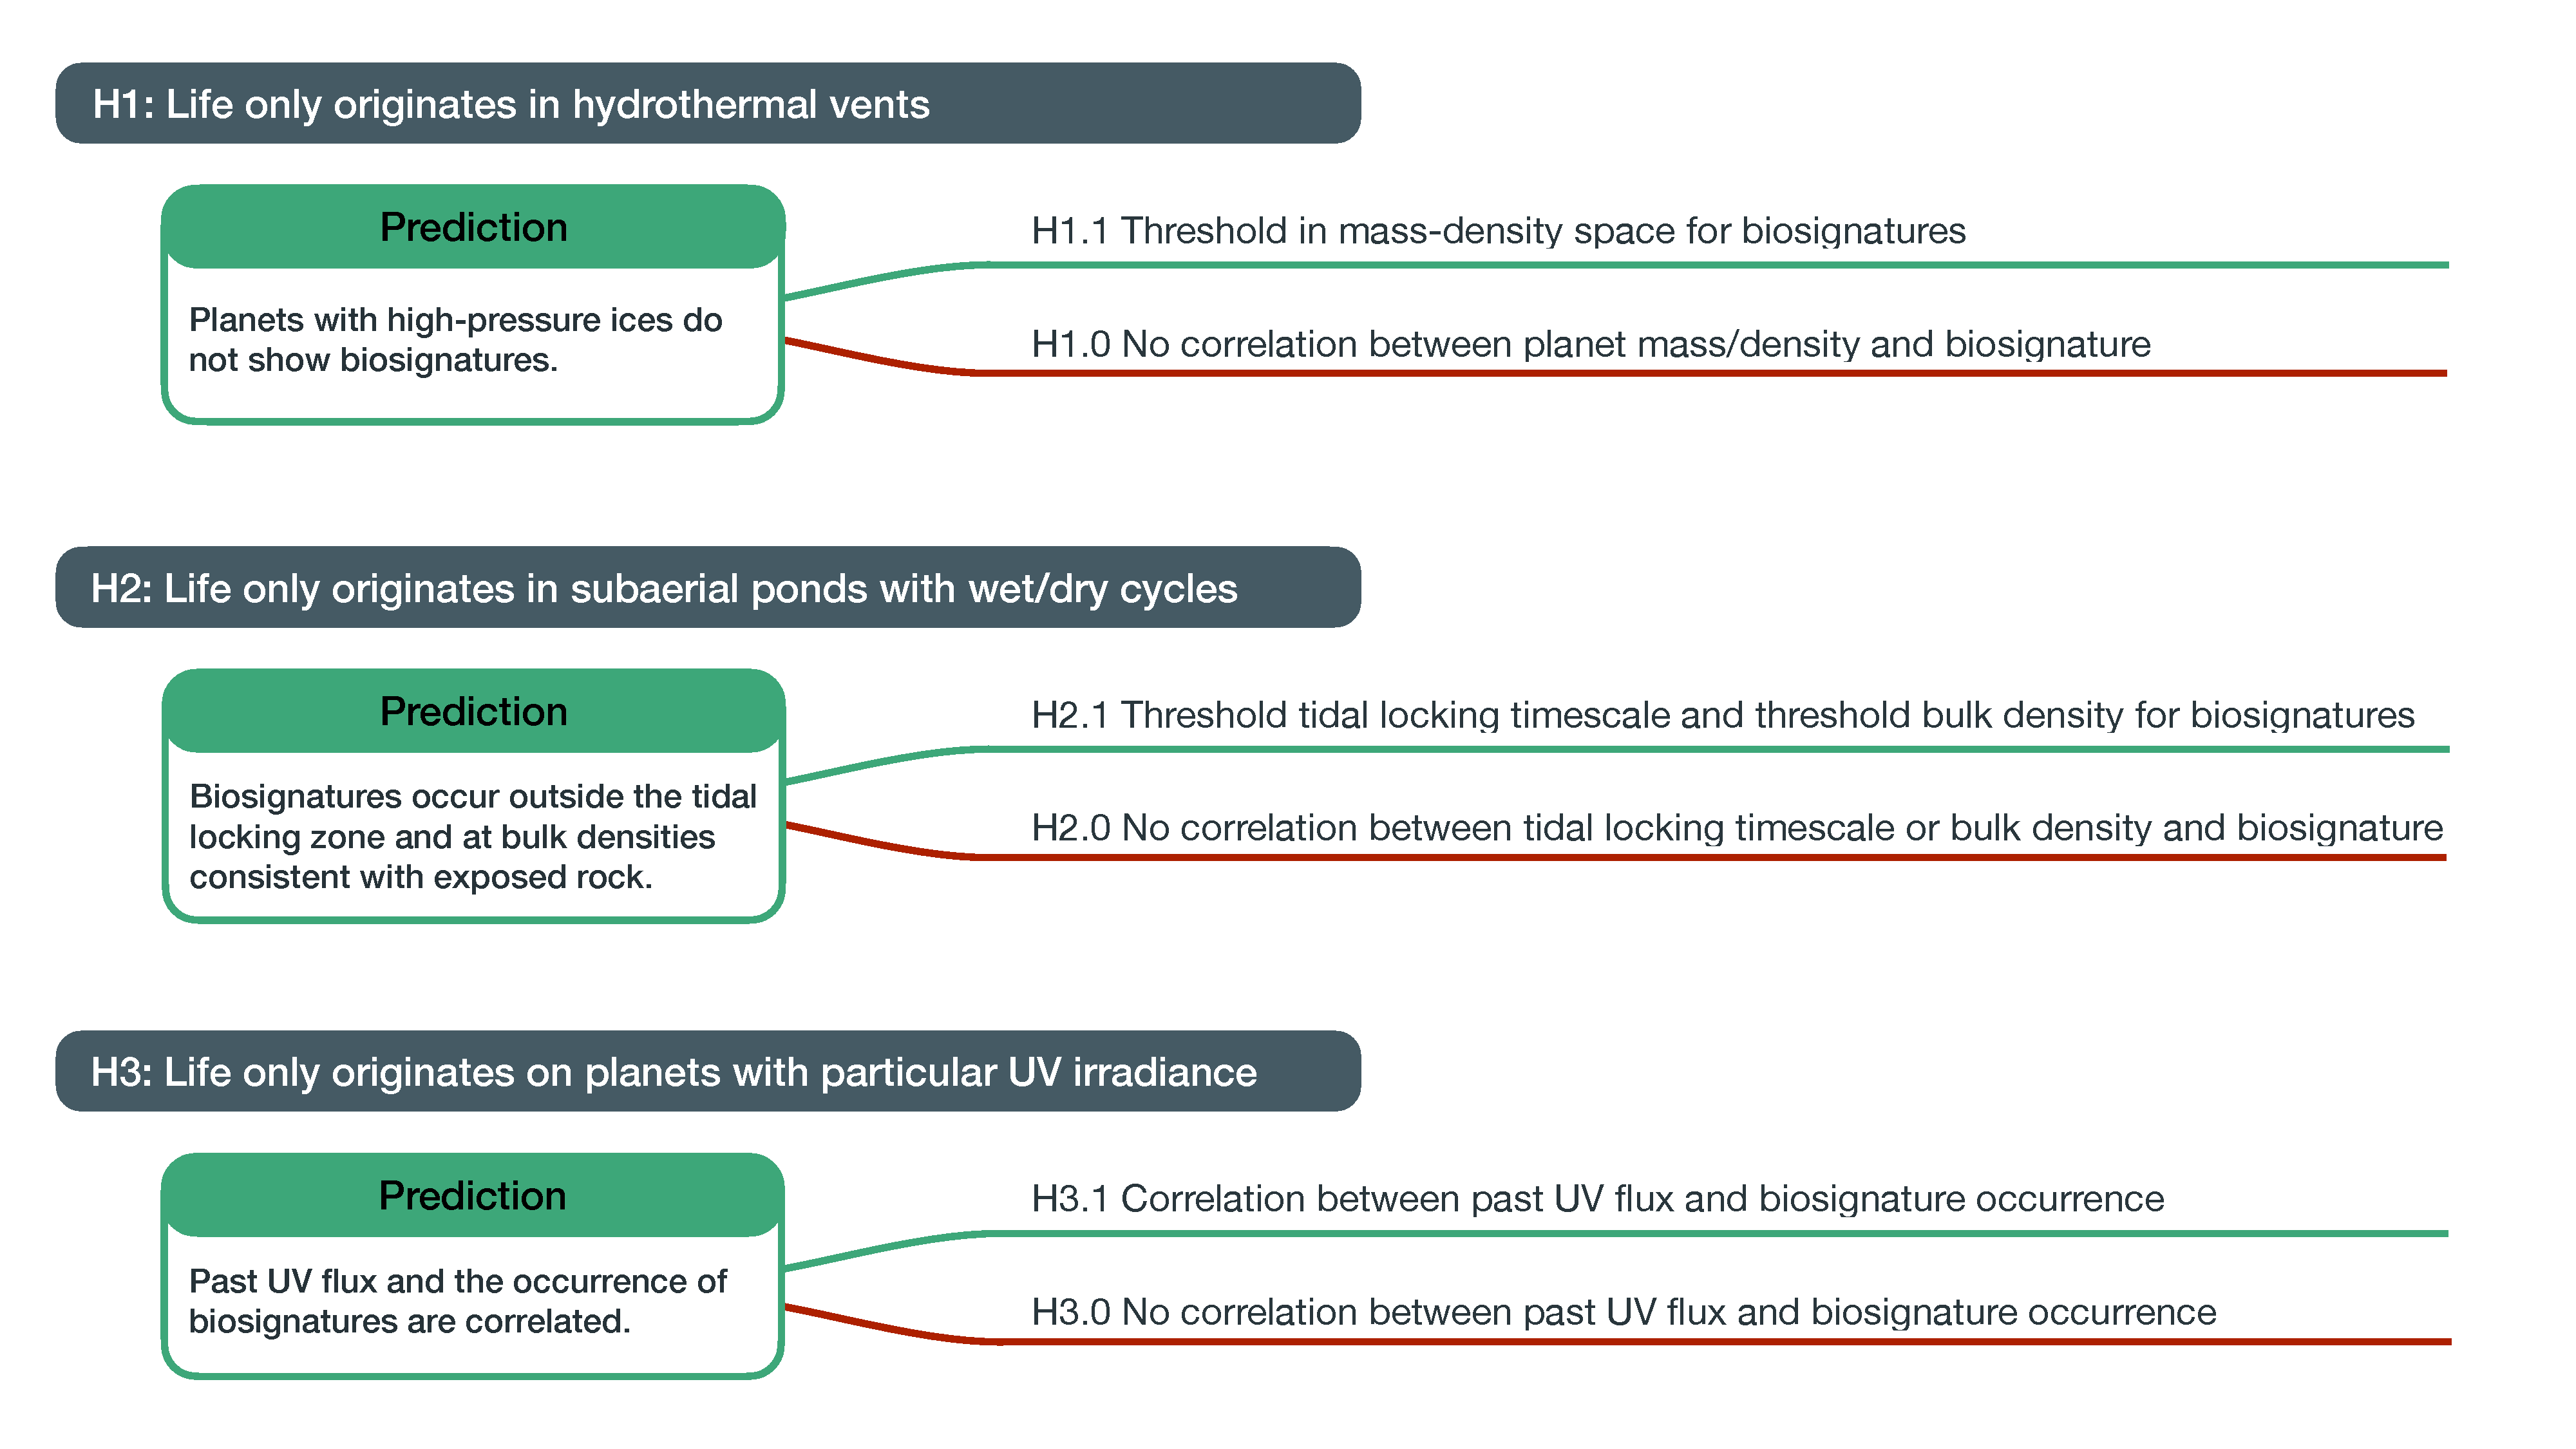
\includegraphics[width=\hsize]{figures/hypotheses.pdf}
        \caption{UV~Threshold Hypothesis and null hypothesis derived from the cyanosulfidic scenario.}
        \label{fig:hypotheses}
    \end{centering}
\end{figure*}
Figure~\ref{fig:hypotheses} shows these hypotheses as derived from the predictions of the cyanosulfidic scenario.
Given a sample of planets, where for some of them we have convincing biosignature detections but remain agnostic on $f_\mathrm{life}$, we ask what evidence for $H_1$ and $H_\mathrm{null}$ we can expect to obtain.

A real exoplanet survey will be subject to observational biases and sample selection effects, and will be constrained by the underlying demographics of the planet sample.
To assess the information gain of a realistic exoplanet survey, we employed \bioverse~\citep{Bixel2021,Hardegree-Ullman2023,Schlecker2024,Hardegree-Ullman2024}, a framework that integrates multiple components including statistically realistic simulations of exoplanet populations, a survey simulation module, and a hypothesis testing module to evaluate the statistical power of different observational strategies.

%\textbf{Prediction:} Biosignatures occur outside the tidal locking zone and at bulk densities consistent with exposed rock.
%\todo[inline]{SR: I'm not a priori sold that tidal locking means that no wet-dry cycles occur. you can still have cycling driven by transient changes in instellation due to flares, for example (e.g., https://iopscience.iop.org/article/10.3847/1538-4357/aadfd1/meta). Similarly, I wonder if 3D effects might not give rise to variability (https://iopscience.iop.org/article/10.3847/PSJ/acc9c4/meta).  I argue that it is more robust to establish a correlation between biosignatures and planets which show evidence of continents/land. I think that Ty Robinson in our department has done some work in this area, his papers might be a good starting point. Other papers which look relevant (but with which I am not familiar, as this is not my area): https://academic.oup.com/mnras/article/511/1/440/6501216, https://academic.oup.com/mnras/article/495/1/1/5733176, https://iopscience.iop.org/article/10.3847/1538-3881/aad775/meta, https://iopscience.iop.org/article/10.3847/1538-3881/aaed3a/meta, https://iopscience.iop.org/article/10.3847/1538-3881/ab2df3/meta}


%\subsection{Other Processes related to the Origins of Life}
%\subsubsection{Planetary redox state and evolution}
%The synthesis of prebiotic compounds requires moderately to highly reduced chemical environments (Kitadai \& Maruyama 2018, Benner+2020, Sasselov+2020, Lichtenberg \& Clement 2022).
%...
%Surficial origins of life chemistries are dependent on the redox state of a planet being $\sim$neutral (not too reduced or oxidized) to allow the presence of precursor molecules like HCN. The planetary redox state leaves an imprint on its atmospheric composition and thus planet size (very reduced atmospheres are large) and spectral signatures. Connected to the cyanosulfidic scenario, the pond scenario, and the impact trigger.
%
%\subsubsection{Impact trigger}
%Iron-rich impactors have been suggested to intermittently provide the reduced environments favored by prebiotic chemistry (e.g., Sekine+2003, Hashimoto+2007, Kuwahara \& Sugita 2015, Genda+2017, Wogan+2023).
%...
%Prebiotic synthesis triggered through reduced impactors that stochastically create transiently reducing or neutral atmospheres requires a certain composition of the impactors, the planet to not be in a magma ocean state (???) (Lichtenberg \& Clement 2022), and, related to this requirement, occurrence of impact events during early planetary evolution.
%Suggested observables are stochastic increases in brightness temperature, transient increases of planet size, and change of planet composition (decreasing with decreasing impact rate, i.e., stellar age).

This paper is organized as follows:
In Section~\ref{sec:methods}, we introduce both our semi-analytical approach and \bioverse\ simulations for testing the UV Threshold Hypothesis.
Section~\ref{sec:results} presents the results of these experiments for a generic survey as well as for a realistic transit survey.
In Section~\ref{sec:discussion}, we discuss our findings before concluding with a summary in Section~\ref{sec:conclusions}.

%% check https://psu.mediaspace.kaltura.com/media/David+Kipping/1_30ntfov6
\section{Bayesian Analysis}
%\todo[inline]{consider Fisher matrix (Kendall \& Stuart 1977; Tegmark 1997) analysis to determine sensitivity of a survey to a set of parameters?}
It is instructive to consider the constraining power of a successful biosignature detection for competing OoL scenarios, which we here attempt with an analytical approach.
The hydrothermal vents scenario ($H_1$) and the subaereal pond scenario ($H_2$) can be considered as mutually exclusive models, and we may study how a particular future observation of biosignatures impacts our beliefs about the relative model probabilities.

We may first consider the probability $\pdf(bio|H_i)$ of detecting a convincing biosignature on a planet, given a particular OoL hypothesis $H_i, \, i \in 1, 2$ is true.
This can be decomposed into the probability of abiogenesis in a particular environment $\pdf_\mathrm{env, i}$, the fraction of life-hosting worlds that develop atmospheric biosignatures $\pdf_\mathrm{sig}$, the probability of the planet type required by the OoL hypothesis occurring in the surveyed sample $\pdf_\mathrm{\eta, i}$, and the probability of detecting the biosignature on this planet type with current technology $\pdf_\mathrm{det, i}$, yielding

\begin{align}
    \label{eqn:pbio}
    \pdf(bio|H_i) = \pdf_\mathrm{env, i} \times \pdf_\mathrm{sig} \times \pdf_\mathrm{\eta, i} \times \pdf_\mathrm{det, i}.
\end{align}

However, what we are actually interested in is the probability of a OoL hypothesis being true, given a particular biosignature detection, $\pdf(H_i|bio)$.
To obtain this we can use Bayes' theorem, which yields
\begin{align}
    \pdf(H_i|bio) = \frac{\pdf(bio|H_i) \pdf(H_i)}{\pdf(bio)}.
\end{align}
Here, $\pdf(H_i)$ is the prior probability of the OoL hypothesis $H_i$, and $\pdf(bio)$ is the prior probability of detecting a biosignature.
% Following Eq.~\ref{eqn:pbio}, we can sum over all possible scenarios to obtain
% \begin{align}
% \pdf(bio) = \sum_{i=1}^{N} \pdf_\mathrm{env, i} \times \pdf_\mathrm{sig} \times \pdf_\mathrm{\eta, i} \times \pdf_\mathrm{det, i}.
% \end{align}

If the hypotheses $H_i$ are adjunct, i.e., their joint occurrence is impossible, one can show that
\begin{align}
    \pdf(H_i|bio) = \frac{\pdf(bio|H_i) \pdf(H_i)}{\sum_{i=1}^{N} \pdf(bio|H_i) \pdf(H_i)}.
\end{align}
Then the parameters in Eq.~\ref{eqn:pbio} that are independent of the chosen hypothesis $H_i$ eliminate and we obtain
\begin{align}
    \pdf(H_i|bio) = &\frac{\pdf_\mathrm{env, i} \pdf_\mathrm{\eta, i} \pdf_\mathrm{det, i} \pdf(H_i)}{\sum_{i=1}^{N} \pdf_\mathrm{env, i} \pdf_\mathrm{\eta, i} \pdf_\mathrm{det, i} \pdf(H_i)} \\
    \overset{\pdf(H_i) = \pdf(H_j)}{ \underset{\forall i,j \in \{1, 2\}}{=}} &\frac{\pdf_\mathrm{env, i} \pdf_\mathrm{\eta, i} \pdf_\mathrm{det, i}}{\sum_{i=1}^{N} \pdf_\mathrm{env, i} \pdf_\mathrm{\eta, i} \pdf_\mathrm{det, i}},
\end{align}
where in the last step we made the implicit assumption that all OoL hypotheses are a priori equally probable.

If we take the ratio of these posteriors for our two independent hypotheses $H_1$ and $H_2$, we get the \textit{Bayes Factor}
\begin{align}
    \label{eq:bayesfactor}
    \frac{\pdf(H_1|bio)}{\pdf(H_2|bio)} = \frac{\pdf_\mathrm{env, 1} \pdf_\mathrm{\eta, 1} \pdf_\mathrm{det, 1}}{\pdf_\mathrm{env, 2} \pdf_\mathrm{\eta, 2} \pdf_\mathrm{det, 2}},
\end{align}
which quantifies the evidence of the data arising from $H_1$ versus $H_2$.

% Putting everything together, we arrive at
% \begin{align}
% \label{eqn:posterior}
% \pdf(H_i|bio) = \frac{\pdf(H_i)}{\pdf(bio)} \times \pdf_\mathrm{env, i} \times \pdf_\mathrm{sig} \times \pdf_\mathrm{\eta, i} \times \pdf_\mathrm{det, i}.
% \end{align}
% If we assume that all OoL hypotheses are a priori equally probable, we can treat $\frac{\pdf(H_i)}{\pdf(bio)}$ in Eq.~\ref{eqn:posterior} as a normalization constant.
In the following, we discuss the impact of the remaining variables $\pdf_\mathrm{env, i}$, $\pdf_\mathrm{\eta, i}$ and $\pdf_\mathrm{det, i}$ on the Bayes factor.

\subsection{Required environment $\pdf_\mathrm{env, i}$}
% Following previous work~\citep{Spiegel2012,Chen2018,Kipping2021}, we may adopt a uniform rate model for abiogenesis, i.e., assume that OoL events occur at a uniform rate.
% This corresponds to a Poisson process with a rate parameter $lambda$, where we make the implicit assumption that abiogenesis occurs only via a single, unique mechanism, only once, and instantaneous.
% If this event occurs within a limited time window $t$, say, between planets form around a star and when it leaves the main sequence, we have
% \begin{align}
% \pdf_\mathrm{env, i} = 1 - \exp(-\lambda t).
% \end{align}
% ~\\
\todo[inline]{The planet should be in the liquid-water HZ}
...
Let us assume that $H_1$ only requires a minimum bulk density $\rho_1$, such that $\pdf_\mathrm{env, 1} \rightarrow 1$ for $\rho >> \rho_1$ and $\pdf_\mathrm{env, 1} \rightarrow 0$ for $\rho << \rho_1$.
On the other hand, $H_2$ requires exposed land and thus a small water mass fraction.
We may implement this in the same way as above but with a minimum bulk density $\rho_2 > \rho_1$.
Furthermore, there is a requirement that the tidal locking timescale may not be so small that the planet is likely tidally locked at observation.
This translates to imposing a minimum semimajor axis $a_2$.

To approximate these thresholds including their expected intrinsic fuzziness, we model them with logistic sigmoid functions
\begin{align}
    \pdf_\mathrm{env, 1} &= \frac{1}{1+\exp[-(C  (\rho - \rho_1))]} \quad \mathrm{and}\\
    \pdf_\mathrm{env, 2} &= \frac{1}{1+\exp[-(C  (\rho - \rho_2))]} \times \frac{1}{1+\exp[-(C  (a - a_2))]},
\end{align}
where $C$ is a compression factor characterizing the steepness of the sigmoid function.
\begin{figure}[ht!]
    \script{bayes_rho-a.py}
    \begin{centering}
        \includegraphics[width=\linewidth]{figures/analytic/Penv.pdf}
        \caption{
            Probability of abiogenesis for the OoL hypotheses $H_1$ and $H_2$ as a function of planet bulk density and semi-major axis.
            $H_1$ only requires large enough densities to exclude deep global water oceans.
            $H_2$ requires a higher minimum density due to the exposed land requirement, and small semi-major axes are excluded to prevent tidal locking.
        }
        \label{fig:Penv}
    \end{centering}
\end{figure}
Figure~\ref{fig:Penv} shows the corresponding $\pdf_\mathrm{env}$ factors and where their regions of high probability overlap.

\subsection{Planet occurrence rate $\pdf_{\eta}$}
We model $\pdf_{\eta, i} (a, \rho)$ following the suggested broken power-law occurrence rates from NASA’s Exoplanet Program Analysis Group chartered Science Analysis Group 13 (SAG 13)~\citep[see][]{Bixel2021} and converting between semi-major axis and period, and between bulk density and radius assuming Earth-like orbits and compositions. \todo[inline]{this is an oversimplification.}
\begin{figure}[ht!]
    \script{bayes_rho-a.py}
    \begin{centering}
        \includegraphics[width=\linewidth]{figures/analytic/Peta.pdf}
        \caption{
            Planet occurrence rate density assuming SAG~13 occurrence rates.
        }
        \label{fig:Peta}
    \end{centering}
\end{figure}
The resulting occurrence rate density has a strong preference for low-density planets on short orbits (see Fig.~\ref{fig:Peta}).
\todo[inline]{This assumes the same occurrence rate for both hypotheses. Is this sensible? If yes, it does not impact the Bayes factor (Eq. \ref{eq:bayesfactor}); we could bring it only later to see where high Bayes factor and planet occurrence overlap.}

\subsection{Information content of a biosignature detection}
We may now evaluate Eqn.~\ref{eq:bayesfactor} to measure the information content with respect to favoring $H_1$ versus $H_2$ depending on the position of a planet with a confirmed biosignature detection in density-orbital distance space.
\begin{figure}[ht!]
    \script{bayes_rho-a.py}
    \begin{centering}
        \includegraphics[width=\linewidth]{figures/analytic/bayes_rho-a.pdf}
        \caption{
            Bayes factor (Eqn.~\ref{eq:bayesfactor}) evaluated at different bulk densities and orbital distances.
            Contour levels reflect the empirical scale for strength of evidence suggested by Jeffreys et al. 19XX.
            There, $\ln(\mathcal{B}) = 2.5$ corresponds to ``moderate'' evidence, and $\ln(\mathcal{B}) = 5 $ corresponds to ``strong'' evidence.
            Only short orbits ($a \lessapprox \SI{0.03}{\au}$) and low bulk densities ($\rho \lessapprox \SI{0.6}{\rho_\oplus}$) allow a selection between the proposed models; they lead to a strong preference for hypothesis $H_1$.
            There is no region in this parameter space that provides strong evidence for $H_2$.
        }
        \label{fig:bayes_rho-a}
    \end{centering}
\end{figure}
Figure~\ref{fig:bayes_rho-a} shows the logarithm of the Bayes factor in this space, providing a scale for evaluating the strength of evidence to prefer one of the proposed models.
Only a small region allows for a significant model selection: While short orbits ($a \lessapprox \SI{0.03}{\au}$) and low bulk densities ($\rho \lessapprox \SI{0.6}{\rho_\oplus}$) strongly support $H_1$, no combination of bulk density and orbital distance provide strong evidence for $H_2$ over $H_1$ without additional information.
 \todo[inline]{factor in Detection probability P\_det}
 \todo[inline]{TODO: test sensitivity of this result on the assumed function and thresholds for P\_env}




% \subsection{biosignature fraction $\pdf_\mathrm{env, i}$}
% Limiting ourselves to the search for \textit{life-as-we-know-it}, we may assume that there are atmospheric biomarkers present on a planet after the abiogenesis event and until global extinction.

%\subsection{Fractional planet occurrence rate $\pdf_\mathrm{\eta, i}$}
%As the different OoL hypotheses do not all work on the same planet types, we may study the impact of the fractional occurrence rates of different planet types on the posterior probability $\pdf(H_i|bio)$.
%For simplicity, let's consider only planets that allow at least one of the scenarios.
%We also ignore any influence of other planets in the same system, e.g. an outer gas giant that itself does not develop life~\citep{Schlecker2021a} or panspermia scenarios CITE.
%We may then distinguish between:
%\begin{enumerate}
%    \item Earths, i.e., limited-water terrestrial planets in the liquid water habitable zone ($H1, H2$). These planets with roughly Earth-like water mass fractions support both the existence of submarine hydrothermal vents ($H1$) and hydrothermal fields with wet/dry cycles ($H2$). Limits in exoplanet observables to this planet type are their orbital distance (both scenarios require liquid water; at least for FGK stars this requirement also puts the planet outside of the tidal locking zone ($H2$)), and bulk density ($H1$ and $H2$ require limited water fractions).
%    \item ``shallow ocean'' water worlds ($H1$). These planets have no land surface exposed to the atmosphere, thus excluding the subaerial pond scenario.
%    \item ``deep ocean'' water worlds. Through the development of high-pressure ices, these planets do not support any of the considered OoL scenarios.
%\end{enumerate}
%
%
%


\subsection{Detection probability $\pdf_\mathrm{det, i}$}



\subsection{Discussion of Bayesian analysis}

\begin{note}
    shallow ocean planets are vulnerable to water loss through high-energy radiation, limiting the time window for habitability especially if no geochemical feedbacks exist~\citep{Kite2018}.
\end{note}
\todo[inline]{discuss host star spectral type dependencies, e.g., abiogenesis time window for G stars ($\lessapprox 10 Gyr$, MS lifetime) or M dwarfs. \citep[e.g.,][]{Spiegel2012}}








%\subsection{Origins of Life Hypotheses}

\section{Methods}
\label{sec:methods}
%\todo[inline]{Briefly introduce Bayesian model comparison, then present the particular hypotheses in their mathematical form.}

\subsection{Fraction of inhabited planets with detectable biosignatures}
%\subsection{H1: Life only originates in hydrothermal vents}
%The hydrothermal vent scenario does not allow oceans deep enough to form an impenetrable layer of high-pressure ice on its floor.
%The resulting allowed parameter space is described by a lower limit on the bulk density. \todo[inline]{+ exclude atmospheric signature for water worlds?}
%...
%
%\subsection{H2: Life only originates in subaerial ponds with wet/dry cycles}
%We parametrize the required exposed land surface in this scenario as a lower limit in bulk density that is higher than for H1.
%Further, the tidal locking timescale of the planet may not be smaller than the age of the system.
%...
%
%\subsection{H3: Life only originates on planets with particular UV irradiance}
%\todo[inline]{\citet{Guenther2020} relate U-band energy to bolometric flux.}
%\todo[inline]{OPTIONAL: ``We further test the scenario of a linear correlation of past UV flux and biosignature occurrence rate.
%This test requires the detection of multiple biosignatures.''
%~\\
%Test for negative correlations as well?}
Here, we conduct a theoretical experiment on the UV~Threshold Hypothesis by relating the occurrence of life on an exo-earth candidate with a minimum past quiescent stellar \gls{UV} flux, focusing on the prebiotically interesting \gls{NUV} range from \SIrange{200}{280}{\nano\meter}~\citep{Ranjan2016}.
Our core hypothesis shall be that life only occurs on planets that at some point in their history have received such radiation at a flux exceeding a threshold $F_\mathrm{NUV, min}$.


\subsection{Semi-analytical approach}\label{sec:met-semianalytical}
%First, we apply a Bayes Factor Design Analysis~\citep{Schoenbrodt2018}
We first assessed the expected probabilities of obtaining true negative or true positive evidence for the UV Threshold Hypothesis ($H_1$) above, as well as the probability for misleading or inconclusive evidence, under idealized conditions.
This serves as a first-order estimate of the information content of a survey, before we take into account the effects of exoplanet demographics, sample selection, and survey strategy.

Presumably, not all habitable worlds are inhabited and not all inhabited worlds develop detectable biosignatures.
The fraction of \glspl{EEC} that are both inhabited and exhibit detectable biosignatures at the time of observation is unknown \rev{and is represented by the term $f_\mathrm{life}$.
This encompasses the probability of life both emerging and persisting to produce detectable biosignatures.}
Let us consider the probability to detect a biosignature $P(L)$, and let our observable be the inferred past \gls{NUV} flux of the planet $F_\mathrm{NUV}$.
Under Hypothesis $H_1$, there exists a special unknown value of $F_\mathrm{NUV}$, noted $F_\mathrm{NUV, min}$ such that

\begin{align}
    P(L|F_\mathrm{NUV},H_1) &=  f_\mathrm{life} \quad \text{if } F_\mathrm{NUV}>F_\mathrm{NUV, min}\\
    P(L|F_\mathrm{NUV},H_1) &=  0               \quad  \text{otherwise}
\end{align}

where $f_\mathrm{life}$ is the unknown probability of abiogenesis.
The corresponding null hypothesis $H_\mathrm{null}$ is that there exists no such special value of $F_\mathrm{NUV}$ and that
\begin{equation}
P(L|F_\mathrm{NUV},H_\mathrm{null}) = f_\mathrm{life}.
\end{equation}
In other words, $H_\mathrm{null}$ states that $P(L)$ is independent of $F_\mathrm{NUV}$.

Defining a sample of size $n$ as $X=\{F_\mathrm{NUV, i},L_i\}_{i \in [1,n]}$ where $L_i$ is equal to 1 if life is detected and 0 otherwise, we can calculate the evidence for hypothesis $H_i$ being true against $H_j$ through the Bayes factor
\begin{equation}
BF_{H_i,H_j} = \frac{P(X|H_i)}{P(X|H_j)},
\end{equation}
with $P(X|H_i)$ and $P(X|H_j)$ likelihoods of obtaining the sample $X$ under either hypothesis.

Let $Y=\sum_i^n L_i$ be the random variable counting the number of positive life detections in a sample of size $n$. Its probability mass function under the null hypothesis $H_\mathrm{null}$ is that of a binomial distribution:
\begin{equation}
P(Y=k|H_\mathrm{null}) = \binom{n}{k}f_\mathrm{life}^k(1-f_\mathrm{life})^{n-k}.
\end{equation}

Under $H_1$, $Y$ also follows a binomial distribution, however it is conditioned by $n_{\lambda} = n(\{F_\mathrm{NUV, i} \text{ if } F_\mathrm{NUV, i}>F_\mathrm{NUV, min}\}_{i \in [1,n]})$, the number of values of $F_\mathrm{NUV}$ in the experiment that exceed $F_\mathrm{NUV, min}$
\begin{equation}
\label{eq:semian:likelihoodH1}
P(Y=k|H_1) = \binom{n_{\lambda}}{k}f_\mathrm{life}^k(1-f_\mathrm{life})^{n_{\lambda}-k}.
\end{equation}

Hence,
\begin{subequations}
\begin{equation}\label{eq:bayes_factor}
BF_{H_1,H_\mathrm{null}} = \frac{P(Y=k|H_1)}{P(Y=k|H_\mathrm{null})} = \frac{\binom{n_\lambda}{k}}{\binom{n}{k}}(1-f_\mathrm{life})^{n_{\lambda}-n},
\end{equation}
and
\begin{equation}\label{eq:bayes_factor2}
BF_{H_\mathrm{null},H_1} = \frac{P(Y=k|H_\mathrm{null})}{P(Y=k|H_1)} = \frac{\binom{n}{k}}{\binom{n_\lambda}{k}}(1-f_\mathrm{life})^{n-n_{\lambda}}.
\end{equation}
\end{subequations}

Given a sample of planets, where for some of them we have convincing biosignature detections but remaining agnostic on $f_\mathrm{life}$: What evidence for $H_\mathrm{1}$ and $H_\mathrm{null}$ can we expect to get?
The analytical expression for the Bayes factor of this inference problem (Equation~\ref{eq:bayes_factor}) is determined by the unknown variables $f_\mathrm{life}$ and $F_\mathrm{NUV, min}$, as well as by the summary statistic $Y$ (number of biosignature detections).
To compute the distribution of evidences, we repeatedly generated samples under $H_\mathrm{1}$ and $H_\mathrm{null}$ and computed the Bayes factors $BF_{H_1,H_\mathrm{null}}$ and $BF_{H_\mathrm{null}, H_1}$.
We then evaluated the fraction of Monte Carlo runs in which certain evidence thresholds~\citep{Jeffreys1939} were exceeded.

Under a more realistic scenario, the distribution of $n_{\lambda}$ depends on additional planetary properties and their evolution, as well as on observational biases and sample selection effects of the survey.
We will address these in the following section.


\subsection{Exoplanet survey simulations with \bioverse}
To assess the diagnostic power of realistic exoplanet surveys, we employed our survey simulator and hypothesis testing framework \bioverse~\citep{Bixel2021}.
The general approach is as follows:
\begin{enumerate}
\item \textbf{Exoplanet population synthesis:} We populate the Gaia Catalogue of Nearby Stars~\citep{Smart2021} with synthetic exoplanets whose orbital parameters and planetary properties reflect our current understanding of exoplanet demographics~\citep{Bergsten2022,Hardegree-Ullman2023}.
Here, we also inject the demographic trend in question - in this case we assign biosignatures according to $H_1$, i.e., to planets in the \gls{HZ} that have received \gls{NUV} fluxes above a certain threshold.
    \item \textbf{Survey simulation:} We simulate the detection and characterization of these exoplanets with a hypothetical survey, taking into account the survey's sensitivity, target selection, and observational biases.
To model the sensitivity of the information gain of a proposed mission to sample selection and survey strategy, we conduct survey simulations with \bioverse\ using different sample sizes and survey strategies.
    \item \textbf{Hypothesis testing:} We evaluate the likelihood that a given survey would detect a specified demographic trend in the exoplanet population and estimate the precision with which the survey could constrain the parameters of that trend.
    A common definition of the null hypothesis $H_\mathrm{null}$, which is also applied here, is that there is no relationship between the independent variable (here: maximum NUV flux) and the dependent variable (here: biosignature occurrence).
    The alternative hypothesis $H_1$ proposes a specific relationship between the independent and dependent variables.
    \bioverse\ offers either Bayesian model comparison or non-parametric tests to evaluate the evidence for or against the null hypothesis.
\end{enumerate}

To determine the diagnostic capability of a given survey, \bioverse\ runs multiple iterations of the simulated survey and calculates the fraction of realizations that successfully reject the null hypothesis.
We used this metric, known as the statistical power, to quantify the potential information content of the survey, identify critical design trades, and find strategies that maximize the survey's scientific return.
% TODO: IF INFERENCE: add:
%The posterior samples obtained from the nested sampling runs further allows us to estimate the precision with which the survey could constrain the parameters of the hypothesized trend.


\subsubsection{Simulated star and planet sample}
We generated two sets of synthetic exoplanet populations, one for FGK-type stars and one for M-type stars.
The stellar samples are drawn from the Gaia Catalogue of Nearby Stars~\citep{Smart2021} with a maximum Gaia magnitude of \var{M_G_max} and a maximum stellar mass of \var{M_st_max} \SI{}{\Msun}.
We included stars out to a maximum distance $d_{\max}$ that depends on the required planet sample size.
Planets were generated and assigned to the synthetic stars following the occurrence rates and size/orbit distributions of \citet{Bergsten2022}.
Following \citet{Bixel2021}, we considered only transiting \glspl{EEC} with radii $0.8\, S^{0.25} < R < 1.4 $ that are within the \gls{HZ} (see Section~\ref{sec:met-hz}).
The lower limit was suggested as a minimum planet size to retain an atmosphere~\citep{Zahnle2017}.
For all survey simulations and hypothesis tests, we repeated the above in a Monte Carlo fashion to generate randomized ensembles of synthetic star and planet populations~\citep[][]{Bixel2021}.



\subsubsection{Habitable zone occupancy and UV flux}\label{sec:met-hz}
To construct a test the UV~Threshold Hypothesis, we required that life occurs only on planets with sufficient past \gls{UV} irradiation exceeding the origins of life threshold $F_\mathrm{NUV, min}$.
Further, we required this flux to have lasted for a minimum duration $\Delta T_\mathrm{min}$ to allow for a sufficient ``origins timescale''~\citep{Rimmer2023}.
All commonly investigated origins-of-life scenarios require water as a solvent;
we thus considered only rocky planets that may sustain liquid water on their surface, i.e., that occupy their host star's momentary \gls{HZ} during the above period, as well as at the epoch of observation.
To determine \gls{HZ} occupancy, we took into account the evolution of the host star's luminosity and \gls{HZ} boundaries.

The \gls{HZ} describes a region around a star where a planet with Earth's atmospheric composition and climate feedbacks can maintain liquid water on its surface~\citep[e.g.,][]{Ramirez2017,Ramirez2018,MolLous2022,Spinelli2023,Tuchow2023}.
Here, we adopted orbital distance estimates that define the \gls{HZ} as the region between the runaway greenhouse transition, where the stellar instellation cannot anymore be balanced through infrared cooling to space~\citep{Ingersoll1969}, and the maximum greenhouse limit, corresponding to the maximum distance at which surface temperatures allowing liquid water can be maintained through a CO$_2$ greenhouse effect~\citep{Kasting1991,Kasting1993,Underwood2003,Kopparapu2013,Kopparapu2014}.
We used the parametrization in \citet{Kopparapu2014} to derive luminosity and planetary mass-dependent distance limits of the \gls{HZ} $a_\mathrm{inner}$ and $a_\mathrm{outer}$.
\rev{The specific boundaries of the habitable zone are known to be sensitive to the star’s luminosity, spectral type, the planet’s mass, and the planet’s atmospheric properties~\citep[e.g.,][]{Pierrehumbert2011,Ramirez2014,Ramirez2017,Ramirez2018b,Koll2019,Ramirez2018,Ramirez2020,Bonati2021,Chaverot2022,Turbet2023}.
The specific habitable zone limits can therefore be variable.
Here -- to constrain the complexity of this study -- we adopted a conservative approach that uses the commonly used limits.
}

% detecting methanogenic life: Sandora2020, Wang2018, Seeburger2023
% TODO: IF SPECIFIC BIOSIGNATURE: use:
%A commonly discussed biosignature is molecular Oxygen (O$_2$), which on Earth emerged as a byproduct of photosynthesis during the Proterozoic era.
%No individual component of an atmosphere has been identified as a reliable biosignature in isolation~\citep{Seager2016}, and the detection of Oxygen alone will certainly not be sufficient to confirm the presence of life.
%Nevertheless, we focus here on detecting this key absorber as it represents the general inherent observational challenges and trends.

To determine \gls{HZ} occupancy, we interpolated the stellar luminosity evolution grid of \citet{Baraffe1998} using a Clough Tocher interpolant~\citep[][see left panel of Figure~\ref{fig:hz_nuv_evo}]{Nielson1983,Alfeld1984} to compute the evolution of the inner (runaway greenhouse) and outer (maximum greenhouse) edges as a function of planet mass and stellar spectral type~\citep{Kopparapu2014}.
Being a local interpolation method, Clough Tocher enables rapid processing while producing a smooth interpolating surface that highlights local trends.
From this, we get each planet's epochs within and outside the \gls{HZ}.

For the \gls{NUV} flux, we used the age- and stellar mass-dependent \gls{NUV} fluxes in the \gls{HZ} obtained by \citet{Richey-Yowell2023}, which considers GALEX \gls{UV} data in the wavelength range of \SIrange{177}{283}{\nano\meter}.
We linearly interpolate in their measured grid, where we convert spectral type to stellar mass using the midpoints of their mass ranges (\SI{0.75}{\Msun} for K~stars, \SI{0.475}{\Msun} for early-type M~stars,  and \SI{0.215}{\Msun} for late-type M~stars).
Outside the age and stellar mass range covered in \citet{Richey-Yowell2023}, we extrapolate using nearest simplex (see right panel of Figure~\ref{fig:hz_nuv_evo}).

We then determined which planets were both in the \gls{HZ} and had \gls{NUV} fluxes above $F_\mathrm{NUV, min}$.
To avoid considering short transitional phases, we require this situation to last for a minimum duration $\Delta T_\mathrm{min} \geq \var{deltaT_min}\,\SI{}{\mega\year}$.
We assigned the emergence \rev{and persistence} of life to a random fraction $f_\mathrm{life}$ of all temperate planets fulfilling these requirements.
For the probability of a planet having detectable biosignatures, $P(\mathrm{bio})$, the UV~Threshold Hypothesis then states
\begin{equation}\label{eq:hypothesis-uv}
    H_{1} : P(\mathrm{bio}) =
        \begin{cases}
            0 , & F_\mathrm{NUV} < F_\mathrm{NUV, min}\\
            f_\mathrm{life}, & F_\mathrm{NUV} \geq F_\mathrm{NUV, min} \\
            & \text{and in HZ for} \, \Delta t \geq \var{deltaT_min} \,\SI{}{\mega\year}
        \end{cases}
\end{equation}
and the corresponding null hypothesis
%\begin{equation}
$H_\mathrm{null} : P(\mathrm{bio}) = f_\mathrm{life},$
%\end{equation}
i.e., no correlation with \gls{UV} flux.
% TODO: IF INFERENCE: add:
%Our choice of priors was to sample $f_\mathrm{life}$ from a log-uniform distribution between $10^{-3}$ and $1$ and $F_\mathrm{NUV, min}$ from a log-uniform distribution between $10^{1}$ and $10^{5}$.

\begin{figure*}
    \script{hz_nuv_evo.py}
    \begin{centering}
        \includegraphics[width=\hsize]{figures/hz_nuv_evo}
%        \includegraphics[width=\hsize]{figures/hz_nuv_evo.bak.png}
        \caption{Interpolated stellar luminosity evolution (left) and evolution of the \gls{NUV} flux in the \gls{HZ} (right) as a function of host star mass.
        Scatter points show age and host star mass of the transiting planets in the synthetic planet sample; crosses denote the estimated \gls{NUV} values in \citet{Richey-Yowell2019}. % with \gls{EEC} highlighted in green.
        We show three evolutionary tracks for a threshold flux of $F_\mathrm{NUV, min} = \var{NUV_thresh}\,\SI{}{\erg\per\second\per\centi\meter\squared}$ that occupy the \gls{HZ} (yellow sections) and exceed the threshold \gls{NUV} flux (red sections) at different times.
        Where these sections overlap (white rectangles), the requirements for abiogenesis are met and we assign a biosignature detection with probability $f_\mathrm{life}$.
        Planet~1 is an \gls{EEC} orbiting a K~dwarf that never receives sufficient \gls{NUV} flux for abiogenesis.
        Planet~2 and Planet~3 enter the \gls{HZ} at different times and receive sufficient \gls{NUV} flux for different durations until their respective host star evolves below the threshold.
        }
        \label{fig:hz_nuv_evo}
    \end{centering}
\end{figure*}



\subsubsection{Transit survey simulations}
With the synthetic star and planet samples generated, we used \bioverse's survey module to simulate noisy measurements of key observables with a transit survey.
We assumed a hypothetical mission that can target a large planet sample with high photometric precision and conduct a biosignature search on these planets~\citep[e.g.,][]{Apai2019,Apai2022}.
The simulated survey was designed to measure planetary instellation (for \gls{HZ} occupancy) with a precision of \var{nautilus_S} and host star effective temperature with a precision of \var{nautilus_T_eff_st}~K.
The maximum past \gls{NUV} flux a planet received can be determined within a precision of \var{nautilus_max_nuv}.
To marginalize over choices of biosignatures and their detectability, which are beyond the scope of this study, we assumed that any inhabited planet would show a biosignature detectable by the survey.

%\subsubsection{Direct imaging survey (e.g., Habitable Worlds Observatory, LIFE)}
%\subsubsubsection{target list}
%\todo[inline]{Provisional stellar target List for the habitable Worlds Observatory:~\citep{Mamajek2023}} % read like in https://github.com/mkenworthy/HWObows/tree/40b1e5f2bc2bbbe8c999b097c80ca5a8cda0aeae/src/scripts

\subsubsection{Hypothesis testing}
%To evaluate the evidence for correctly rejecting the null hypothesis, we employed the Mann-Whitney U test~\citep{Mann1947}.
\rev{We ought to choose a statistical test that is sensitive to the UV~Threshold Hypothesis, and that could be realistically conducted in a future transit survey (which may include auxiliary information from ground-based observations, archived data, or models).
Given the available types of data expected from such surveys, our test shall be non-parametric and compare two samples -- planets with and without biosignatures -- to assess whether they are drawn from the same underlying population in terms of their infered historic maximum NUV flux.
Common options include the Kolmogorov-Smirnov test, the Brunner-Munzel test~\citep{Brunner2000}, and the Mann-Whitney U test~\citep{Mann1947}.
Due to its availability and suitability for large sample sizes, we chose the Mann-Whitney U test, which evaluates if one sample is stochastically greater than the other.
Here, we }
compare the distributions of \gls{NUV} fluxes of planets with and without biosignatures.
The implementation in \bioverse\ relies on the \texttt{scipy.stats.mannwhitneyu} function~\citep{Virtanen2020} and returns a p-value \rev{for each test.
To balance the trade-off between Type I and Type II error risks, we set the significance level to the widely adopted threshold $\alpha = 0.05$.
%This choice ensures a reasonable trade-off between detecting a potential dependence of biosignatures on NUV flux while controlling for statistical noise.
To quantify the diagnostic power of the survey, we conducted repeated randomized realizations and calculated the fraction of successful rejections of the null hypothesis, i.e., the statistical power.
}


\section{Results}
\label{sec:results}
%\subsection{Information content in mass-density space}
%\subsection{Information content in tidal locking timescale-density space}

%\subsection{Correlation of past UV flux and biosignature occurrence}\label{sec:results_uv}

\subsection{Semi-analytical assessment}\label{sec:results-semianalytical}
In Section~\ref{sec:met-semianalytical}, we computed the probability for true positive evidence for $H_\mathrm{1}$ and $H_\mathrm{null}$, respectively (Equations~\ref{eq:bayes_factor},~\ref{eq:bayes_factor2}).
Figure~\ref{fig:semian_true_evidence} shows how these evidences are distributed for sample sizes \var{semian_Nsamp1} and \var{semian_Nsamp2}, and how likely we are to obtain strong evidence ($BF_{H_i, H_j}$ > 10).
For $n = \var{semian_Nsamp1}$, strong true evidence for $H_\mathrm{1}$ ($H_\mathrm{null}$) can be expected in $\sim \SI{30}{\percent}$ ($\sim \SI{40}{\percent}$) of all random experiments.
In the majority of cases, the outcome of the survey will be inconclusive.
\begin{figure*}
    \script{semian_true_evidence.py}
    \begin{centering}
        \includegraphics[width=\hsize]{figures/semian_true_evidence}
        \caption{Obtaining true strong evidence with different sample sizes. Left: Probability to reach given evidence levels for $H_\mathrm{1}$ and $H_\mathrm{null}$ under sample sizes $n = \var{semian_Nsamp1}$ (solid) and $n = \var{semian_Nsamp2}$ (dashed). Vertical lines denote thresholds for ``strong'' evidence, $BF_{H_i, H_j}$ > 10, and ``extreme'' evidence, $BF_{H_i, H_j}$ > 100. Right: Probability of obtaining true strong evidence for $H_\mathrm{1}$ as a function of sample size $n$.}
        \label{fig:semian_true_evidence}
    \end{centering}
\end{figure*}
The situation improves with larger samples: for $n = \var{semian_Nsamp2}$, \SI{80}{\percent} of random samples permit conclusive inference (strong true evidence) under either $H_\mathrm{1}$ or $H_\mathrm{null}$.

The expected resulting evidence further depends on the a priori unknown \rev{rate of life's emergence and persistence} $f_\mathrm{life}$ and on the \gls{NUV} flux threshold.
\begin{figure*}
    \script{semian_true_evidence.py}
    \begin{centering}
        \includegraphics[width=\hsize]{figures/semian_evidence-grid}
        \caption{Probability of obtaining true strong evidence for different abiogenesis rates, \gls{NUV} flux thresholds, and sample sizes. For each of these parameters, higher values increase the probability of yielding strong evidence.}
        \label{fig:semian_evidence-grid}
    \end{centering}
\end{figure*}
Figure~\ref{fig:semian_evidence-grid} illustrates this dependency: For very low values of either parameter, samples drawn under the null or alternative hypotheses are indistinguishable and the Bayesian evidence is always low.
Both higher $f_\mathrm{life}$ and higher \gls{NUV} flux thresholds increase the probability of obtaining strong evidence.
Larger sample sizes enable this at lower values of these parameters.


So far, we have assumed random, uniform distributions of $f_\mathrm{life}$, $F_\mathrm{NUV, min}$, and $F_\mathrm{NUV}$. % Actually it is more than just NUV, it is whatever index that integrates NUV and HZ requiremetns into a single scalar variable for which a threshold exist
A high biosignature detection rate $f_\mathrm{life}$ increases the evidence (see Equation~\ref{eq:bayes_factor}) but a survey strategy cannot influence it.
The same is true for $F_\mathrm{NUV, min}$, where again higher values increase the evidence as the binomial distribution for $H_\mathrm{1}$ gets increasingly skewed and shifted away from the one for $H_\mathrm{null}$.
However, one might select exoplanets for which a biosignature test is performed based on \textit{a priori} available contextual information~\citep{catling2018exoplanet} in order to maximize the science yield of investing additional resources.
For instance, the distribution of $F_\mathrm{NUV}$ in the planet sample can be influenced by the survey strategy, and a targeted sampling approach could favor extreme values. % of $F_\mathrm{NUV}$ in the sample selection.
We model this by distributing $F_\mathrm{NUV}$ according to different $Beta$ functions and introduce a selectivity parameter $s\in]-1,1[$ such that $F_\mathrm{NUV} \sim Beta(1/10^s,1/10^s)$.
Figure~\ref{fig:semian_selectivity} shows how the probability of obtaining true strong evidence for $H_\mathrm{1}$ scales with selectivity $s$.
%Here, $s=0$ corresponds to a random uniform distribution.
%Compared to this case, a high selectivity ($s \sim 1$) can increase the probability of obtaining true strong evidence to $\gtrsim \SI{85}{\percent}$ for large samples.
For large samples, a high selectivity ($s \sim 1$) can increase the probability of obtaining true strong evidence from $\sim \SI{70}{\percent}$ for $s= 0$ (random uniform distribution) to $> \SI{90}{\percent}$.

\begin{figure*}
    \script{semian_true_evidence.py}
    \begin{centering}
        \includegraphics[width=\hsize]{figures/semian_selectivity}
        \caption{Scaling of the probability of obtaining true strong evidence with sample selectivity. Left: Sampling distribution for different selectivity parameters $s$. Right: Resulting \mbox{P(true strong evidence)}, where $f_\mathrm{life}$ and $F_\mathrm{NUV, min}$ are randomly drawn from a uniform distribution. Sampling more extreme values of $F_\mathrm{NUV}$ is more likely to yield strong evidence.}
        \label{fig:semian_selectivity}
    \end{centering}
\end{figure*}




\subsection{Survey simulations with \bioverse}\label{sec:results-bioverse}
%\begin{figure}
%    \script{inhabited_FGKM.py}
%    \begin{centering}
%        \includegraphics[width=\hsize]{figures/inhabited_FGKM}
%        \caption{Host stars of all transiting \glspl{EEC} and inhabited planets in a simulated transit survey.
%        In the FGK sample, most \glspl{EEC} and all inhabited planets orbit K~dwarfs.
%        In an M~dwarf sample of the same size, the fraction of inhabited planets is larger.
%        }
%        \label{fig:inhabited_FGKM}
%    \end{centering}
%\end{figure}
%In a magnitude- and volume-limited sample of a transit survey, the host star distribution for \glspl{EEC} will be skewed toward later spectral types and dominated by M~dwarfs due to how the \gls{HZ} scales with spectral type.
With \gls{HZ} occupancy as a requirement for abiogenesis, and barring selection biases beyond stellar brightness, the host star distribution of inhabited planets in a simulated transit survey is skewed toward later spectral types.
For a fixed planet sample size, the fraction of inhabited planets is highest for planets orbiting M~dwarfs due to the higher \gls{NUV} fluxes in the \gls{HZ} of these stars (see Figures~\ref{fig:hz_nuv_evo},~\ref{fig:surveys_FGKM}).
Their \gls{NUV} fluxes are generally highest at early times $\lesssim\SI{100}{\mega\year}$.
These host stars, in particular late subtypes, also provide extended periods of increased \gls{NUV} emission that overlap with times when some of these planets occupy the \gls{HZ} (see Figure~\ref{fig:hz_nuv_evo}), our requirement for abiogenesis (see Equation~\ref{eq:hypothesis-uv}).
Thus -- under the UV Threshold Hypothesis -- most inhabited transiting planets in the sample orbit M~dwarfs.

Here, we are interested in the statistical power of a transit survey with a plausible sample selection and size.
In the following, we fix the sample size to \var{N_nautilus} and consider two different survey strategies targeting FGK and M~dwarfs, respectively.
We further investigate the sensitivity of the survey to the a priori unknown threshold \gls{NUV} flux $F_\mathrm{NUV, min}$ and the \rev{probability of life emerging and persisting} $f_\mathrm{life}$.

\subsubsection{Selectivity of simulated transit surveys}
In Section~\ref{sec:results-semianalytical}, we showed that the probability of obtaining true strong evidence for the hypothesis that life only originates on planets with a minimum past \gls{NUV} flux is sensitive to the distribution of sampled past \gls{NUV} fluxes, i.e., the selectivity of the survey (compare Figure~\ref{fig:semian_selectivity}).
%The maximum \gls{NUV} distribution of our generic transit survey is rather unimodal with a median around \SI{500}{\erg\per\second\per\centi\meter\squared} (see Figure~\ref{fig:surveys_FGKM}), leading to a selectivity of roughly \var{selectivity_transit_volumelim}.
For both surveys targeting M dwarfs and those targeting FGK dwarfs, the maximum \gls{NUV} distribution is rather unimodal.
Applying the approach from Sect.~\ref{sec:results-semianalytical} of fitting a Beta function to the distribution, we find rather low selectivities (see Figure~\ref{fig:surveys_FGKM}), which is likely detrimental for statistical hypothesis tests.

%\begin{figure*}
%    \script{nuv_distribution.py}
%    \begin{centering}
%        \includegraphics[width=\hsize]{figures/nuv_distribution}
%        \caption{Distribution of maximum past \gls{NUV} flux in transit surveys targeting \glspl{EEC} around FGK and M~stars, respectively. The best-fit beta distributions (gray) correspond to selectivities of $s_\mathrm{FGK} = $\var{selectivity_FGK} and $s_\mathrm{M} = $\var{selectivity_M}. Red areas show inhabited planets for a threshold \gls{NUV} flux of $F_\mathrm{NUV, min} = \var{NUV_thresh}\,\SI{}{\erg\per\second\per\centi\meter\squared}$ and an abiogenesis rate of $f_\mathrm{life} = \var{f_life}$.}
%        \label{fig:nuv_distribution}
%    \end{centering}
%\end{figure*}

\begin{figure*}
    \script{surveys_FGKM.py}
    \begin{centering}
        \includegraphics[width=\hsize]{figures/surveys_FGKM}
        \caption{
        Simulated transit surveys targeting FGK and M~stars.\\
        Top: Host stars of all transiting \glspl{EEC} and inhabited planets in a simulated transit survey.
        In the FGK sample, all \glspl{EEC} and all inhabited planets orbit K~dwarfs.
        In an M~dwarf sample of the same size, the fraction of inhabited planets is larger.\\
        Center: Distribution of inferred maximum past \gls{NUV} flux in transit surveys targeting \glspl{EEC} around FGK and M~stars, respectively. The best-fit beta distributions correspond to selectivities of $s_\mathrm{FGK} = $\var{selectivity_FGK} and $s_\mathrm{M} = $\var{selectivity_M}. Red areas show inhabited planets for an abiogenesis rate of $f_\mathrm{life} = \var{f_life}$ and a generic threshold \gls{NUV} flux $F_\mathrm{NUV, min} = \var{NUV_thresh}\,\SI{}{\erg\per\second\per\centi\meter\squared}$.\\
        Bottom: Recovered biosignature detections and non-detections of simulated transit surveys. The dashed line denotes $F_\mathrm{NUV, min}$.}
        \label{fig:surveys_FGKM}
    \end{centering}
\end{figure*}



\subsubsection{Expected biosignature pattern}
A representative recovery of the injected biosignature pattern is shown in Figure~\ref{fig:surveys_FGKM}.
There, we assumed an abiogenesis rate of $f_\mathrm{life} = \var{f_life}$ and a minimum \gls{NUV} flux of $F_\mathrm{NUV, min} = \var{NUV_thresh}\,\SI{}{\erg\per\second\per\centi\meter\squared}$.
All injected biosignatures are assumed to be detected without false positive ambiguity, and the maximum \gls{NUV} flux is estimated from the host star's spectral type and age with an uncertainty corresponding to the intrinsic scatter in the \gls{NUV} fluxes in \citet{Richey-Yowell2023}.
%\begin{figure*}
%    \script{detections_uv.py}
%    \begin{centering}
%        \includegraphics[width=\hsize]{figures/detections_uv}
%        \caption{Recovered biosignature detections in the \gls{NUV} flux-biosignature occurrence space. The dashed line denotes a generic threshold \gls{NUV} flux $F_\mathrm{NUV, min} = \var{NUV_thresh}\,\SI{}{\erg\per\second\per\centi\meter\squared}$.}
%        \label{fig:detections_uv}
%    \end{centering}
%\end{figure*}
This leads to a distribution of biosignature detections with detections increasingly occurring above a threshold inferred NUV flux.
In this example case, the few biosignature detections in the FGK sample lead to a higher evidence %($dlnZ_\mathrm{FGK} = \var{dlnZ_FGK}$)
than in the M dwarf sample%($dlnZ_\mathrm{M} = \var{dlnZ_M}$)
, where the majority of planets are above the threshold \gls{NUV} flux.


\begin{figure}
    \script{inhabited_aafo_nuv_thresh.py}
    \begin{centering}
        \includegraphics[width=\hsize]{figures/inhabited_aafo_nuv_thresh}
        \caption{Fraction of inhabited planets for different threshold \gls{NUV} fluxes under the UV~Threshold Hypothesis if the abiogenesis rate $f_\mathrm{life} = 1$.
        %Shaded regions denote 90 percent confidence intervals of randomized sample generations, and dashed lines correspond to samples including non-transiting planets.
        For all samples, the fraction of inhabited planets drops sharply with increasing threshold \gls{NUV} flux due to the combined effects of never receiving sufficient \gls{NUV} flux for abiogenesis or receiving it before entering the \gls{HZ}.}
        \label{fig:inhabited_aafo_nuv_thresh}
    \end{centering}
\end{figure}
Figure~\ref{fig:inhabited_aafo_nuv_thresh} shows the fraction of inhabited planets under the UV~Threshold Hypothesis for different threshold \gls{NUV} fluxes and for the limiting case of \rev{a probability for life's emergence and persistence} of $f_\mathrm{life} = 1$.
This fraction decreases sharply with increasing threshold flux, as fewer planets receive sufficient \gls{NUV} flux for abiogenesis.
Another effect responsible for this drop is that some planets receive the required \gls{NUV} flux only before entering the \gls{HZ} -- this is especially likely for M~dwarfs.
For the FGK sample, the fraction of inhabited planets drops at lower threshold fluxes than for the M dwarf sample.


\subsubsection{Statistical power and sensitivity to astrophysical parameters}\label{sec:results-powergrid}
We now investigate the sensitivity of the achieved statistical power of our default transit survey to the a priori unconstrained threshold \gls{NUV} flux $F_\mathrm{NUV, min}$ and the abiogenesis \rev{and persistence} rate $f_\mathrm{life}$.
Figure~\ref{fig:powergrid} shows the statistical power as a function of these parameters for a sample size of $N=\var{N_nautilus}$.
Values of $F_\mathrm{NUV, min}$ that lie between the extrema of the inferred maximum \gls{NUV} flux increase the achieved statistical power of the survey, as in this case the dataset under the alternative hypothesis $H_1$ differs more from the null hypothesis.
Furthermore, \rev{higher $f_\mathrm{life}$ increase} the evidence for $H_1$.

Parameter space regions with statistical power above \SI{90}{\percent} lie at \rev{$f_\mathrm{life} > 0.5$} and mostly at threshold \gls{NUV} fluxes of $\sim \SIrange{200}{400}{\erg\per\second\per\centi\meter\squared}$.
Notably, the sensitivity of the M~dwarf sample extends into the low \gls{NUV} flux end due to the broader distribution of maximum past \gls{NUV} fluxes in this sample.
Here, the FGK sample is barely sensitive.


\begin{figure*}
    \script{powergrid.py}
    \begin{centering}
        \includegraphics[width=\hsize]{figures/powergrid}
        \caption{Statistical power as a function of threshold \gls{NUV} flux and abiogenesis rate. Even for a large sample (here: $N=\var{N_nautilus}$), a high statistical power of the transit survey requires high \rev{rates of life emerging and persisting} $f_\mathrm{life}$.
         Intermediate values of $F_\mathrm{NUV, min}$ are more likely to yield strong evidence than extreme values. \rev{For $f_\mathrm{life} \gtrsim \SI{80}{\percent}$}, the sensitivity of the M~dwarf sample extends into the low \gls{NUV} flux end.
         }
        \label{fig:powergrid}
    \end{centering}
\end{figure*}



\section{Discussion}
\label{sec:discussion}
A key question in the quest to understand the origins of life is which natural processes best explain how living matter spontaneously appears from nonliving matter~\citep[e.g.,][]{Malaterre2022}.
Using astronomical methods, this question will likely not be testable for individual planets but rather for ensembles of planets.
The cyanosulfidic scenario for the origins of life~\citep{Patel2015}, in particular its predicted existence of a minimum \gls{NUV} flux required for prebiotic chemistry, offers an opportunity to test an origins of life hypothesis with a statistical transit survey sampling planets with varying \gls{NUV} flux histories.
In the following, we discuss the prospects of testing the UV~Threshold Hypothesis in light of our results.

\subsection{Sampling strategy for testing a \gls{NUV} flux threshold} % corresponds to conclusion point 1
In Sect.~\ref{sec:results-semianalytical}, we show that testing the UV~Threshold Hypothesis suffers from `nuisance' parameters that hamper inference through astronomical observations.
Here, these parameters are the unspecified value of the \gls{NUV} threshold hypothesized to exist under $H_1$, and the unknown probability of detectable life emerging on a habitable planet $f_{\mathrm{life}}$.
While the inference of a planet's entire \gls{UV} flux evolution is difficult~\citep[e.g.,][]{Richey-Yowell2023}, the estimated maximum \gls{NUV} flux that a planet was exposed to may be used as a proxy, at least if one is interested in a minimum threshold flux and makes the assumption that planetary surfaces offer protection against \textit{too high} UV flux.
Indeed, the distribution of the number of planets with detected biosignature in a particular sample of planets with inferred maximum \gls{NUV} values $F_{\mathrm{NUV}}$ depends on both the values of $F_{\mathrm{NUV},min}$ and $f_{\mathrm{life}}$ as shown in equation~\ref{eq:semian:likelihoodH1}.
%Avoiding a loss in statistical power due to nuisance parameters is a common difficulty in statistical testing, and is the motivation behind elaborate test statistics.

In our semi-analytical analysis (Section~\ref{sec:results-semianalytical}), we project a possible test performed by a future observer equipped with a sample of exoplanets with derived past maximum \gls{NUV} exposure for which biosignature detection has been attempted.
This is necessarily reductive as this observer will have more knowledge about experimental conditions and will therefore be able to use this information to guide hypothesis testing.
For instance, we have made the choice to consider the total number of detected biosignatures as our summary statistic (Equation~\ref{eq:semian:likelihoodH1}), which is not sufficient to infer $F_{\mathrm{NUV},min}$ and $f_{life}$ separately.
However, by conditioning the Bayes factor to these variables (Equation~\ref{eq:bayes_factor}), we calculate the probability distribution of the Bayesian evidence in favor of $H_1$.
In doing so, we may evaluate how evidence depends on the uncertainty over these unknown parameters in general terms, without assuming which particular test a future observer might actually choose to perform over real data when available.
From this, we can see that target selection can strongly affect the conclusiveness of a future test of the UV~Threshold Hypothesis.

%The particular finding that our future observer might prefer to prioritize extreme values of this variable in order to maximize statistical power.
The particular finding that prioritizing extreme values of past \gls{NUV} flux can enhance statistical power likely clashes with observational constraints, as the composition of the subset of planets that we can observe and for which detection of biosignature can be attempted is not independent from their \gls{NUV} flux history.
Hence, for our future observer, selectivity and sample size may be in conflict.
This trade-off can be quantified in terms of expected evidence yield, which we have done in Section~\ref{sec:results-semianalytical}.
Our analysis shows that regardless of selectivity, sample sizes smaller than 50 likely result in inconclusive tests, and that increasing selectivity towards extreme $F_{\mathrm{NUV}}$ offers limited inference gains compared to the uniform case ($s=0$; Figure~\ref{fig:semian_selectivity}).
For larger samples, however, a narrow distribution of $F_{\mathrm{NUV}}$ may prevent inference entirely.
We thus argue that selecting a sample with $F_{\mathrm{NUV}}$ distributed uniformly or emphasizing extreme values should -- barring any practical counterarguments -- be considered in any future attempt at testing the UV~Threshold Hypothesis.
Since the practical implementation of an exoplanet survey can stand in the way of such a selection, the following discussion focuses on the results of our transit survey simulations with \bioverse.

%We stress that a future observer will likely be able to leverage standard frequentist testing methods which may be more likely to yield conclusive results (whether in favor or in disfavor of $H_1$).
%For instance, it would make sense when presented with a sample of planets with various values of $F_{\mathrm{NUV}}$ and for which biosigature detection is attempted to categorize them into two classes: those for which a biosignature is detected, and those for which this is not the case.
%Then, the distribution of $F_{\mathrm{NUV}}$ in each of those categories is compared under the null hypothesis that they are the same.
%In this case, a non-parametric test could be preferred, such as a two-sample Kolmogorov-Smirnov test or perhaps a Mann-Whitney $U$ test.


%\subsection{Constraining power for the origins of life as a function of biosignature location} % corresponds to conclusion points 2, 5
\subsection{How planetary context may constrain the UV~Threshold Hypothesis} % corresponds to conclusion points 2, 5
It comes to no surprise that the success rate for testing the UV~Threshold Hypothesis is sensitive to the sample size of the survey and to the occurrence of life on temperate exoplanets.
As we have shown, the statistical power of this test also depends on the distribution of past \gls{NUV} fluxes in the sample and on the threshold flux.
Optimizing the survey to sample a wide range of NUV flux values, particularly at the extremes, can enhance the likelihood of obtaining strong evidence for or against the hypothesis.
Intermediate values of the threshold \gls{NUV} flux are more likely to yield strong evidence than extreme values, as the dataset under the alternative hypothesis $H_1$ differs more from the null hypothesis in this case while still being sufficiently populated.
The threshold flux is, of course, a priori unknown and we cannot influence it.
If, however, better theoretical predictions for the required \gls{NUV} flux for abiogenesis become available~\citep{Rimmer2021}, the survey strategy can be further optimized, for instance by targeting planets that are estimated to have received a \gls{NUV} flux slightly below and above this threshold or by applying a bisection algorithm in a sequential survey~\citep{Fields2023}.

\subsection{An M~dwarf opportunity}
An interesting aspect lies in the distribution of host star properties, as different spectral types probe different past \gls{NUV} flux regimes.
FGK stars show a narrow distribution of maximum past \gls{NUV} fluxes in the \gls{HZ}, which may -- depending on the (unknown) threshold \gls{NUV} flux -- limit the diagnostic power of a survey.
In the case of a pure FGK sample, it will essentially only be sensitive to \gls{NUV} flux thresholds $\sim \SIrange{200}{400}{\erg\per\second\per\centi\meter\squared}$, and the chance of detecting biosignatures diminishes rapidly for higher thresholds within this range (see Figure~\ref{fig:inhabited_aafo_nuv_thresh}).
Detected biosignatures in an FGK sample would have little constraining power on testing the UV~Threshold Hypothesis; they would either suggest that low NUV fluxes are sufficient for abiogenesis or indicate a different abiogenic pathway~\citep[e.g.,][]{Westall2018}.
A lack of biosignatures in a larger FGK sample would support the UV~Threshold Hypothesis.

On the other hand, M~dwarfs show a wider distribution of maximum past \gls{NUV} fluxes in their \glspl{HZ}.
While old M~dwarfs can be considered low-UV environments, a significant fraction of them emit high \gls{NUV} fluxes into their \gls{HZ} during their early stages, in particular later subtypes~\citep{Richey-Yowell2023}.
This will help to test the high \gls{NUV} flux end of the UV Threshold Hypothesis; a higher occurrence of biosignatures here would support the hypothesis that a higher NUV flux is favorable or necessary for life.
At the same time, a fraction of host stars in our M~dwarf sample extends it to lower maximum past \gls{NUV} fluxes, enabling tests of the low \gls{NUV} flux end of the hypothesis.
The higher and more variable \gls{NUV} fluxes in M~dwarfs thus increase the likelihood of obtaining strong evidence for or against the UV~Threshold Hypothesis.

The combination of a lack of \gls{UV} radiation today, which makes biosignature gases more detectable~\citep{Segura2005}, and a UV-rich past that may have enabled abiogenesis could make M~dwarfs the preferred targets for biosignature searches.
We note that relevant mission concepts, such as the Large Interferometer for Exoplanets~\citep[\life,][]{Quanz2022,Glauser2024}, include M-dwarf systems among their primary targets~\citep{Kammerer2018,Carrion-Gonzalez2023}.
Our findings underscore the importance of constraining the \gls{UV} emission profiles of \gls{EEC} host stars throughout their evolutionary stages to assess the viability of M-dwarf planets as testbeds for theories on the origins of life~\citep{Rimmer2021,Ranjan2023a}.


\subsection{Sensitivity to astrophysical parameters} % corresponds to conclusion point 3
Our \bioverse\ simulations that take into account exoplanet demographics, the evolution of habitability and \gls{NUV} fluxes, and observational biases show that not only the likelihood of a conclusive test of the UV~Threshold Hypothesis, but also the likelihood of successful biosignature detection itself is extremely sensitive to the threshold \gls{NUV} flux if the hypothesis is true.
Even if all biosignatures can be detected and the nominal \rev{rate of life's emergence and persistence} is very high, say $f_\mathrm{life} = 1$, under the condition that prebiotic chemistry requires a minimum \gls{NUV} flux \textit{and} liquid water, if the threshold flux turns out to be high the probability of finding life on a randomly selected planet may be very low.
As we showed, for high required fluxes the two requirements of simultaneous \gls{HZ} occupancy and sufficient \gls{NUV} flux conspire to diminish the fraction of inhabited planets in the sample.
Taking the inferred fluxes from \citet{Richey-Yowell2023} at face value (but taking into account intrinsic scatter), a minimum required \gls{NUV} flux of $\gtrsim\SI{400}{\erg\per\second\per\centi\meter\squared}$ reduces the fraction of inhabited planets to below $\sim\SI{1}{\percent}$.
This not only calls for a large sample size and a targeted sample selection preferring high expected past \gls{NUV} fluxes, but also highlight the necessity of continued theoretical and experimental research into the role of \gls{UV} radiation in prebiotic chemistry~\citep{Ranjan2017b,Rimmer2018,Rimmer2021}.




%\subsection{What do we learn from a single biosignature detection?}
%\todo[inline]{discuss constraining power on OOL of a convincing biosignature detection on a single planet, depending on the position of the planet in the parameter space we explored.}

\subsection{Contextual support for potential biosignature detections} % corresponds to ... which conclusion?
The predicted interplay of \gls{NUV} flux and \gls{HZ} occupancy in enabling abiogenesis via the cyanosulfidic scenario could in principle be used to add or remove credibility from a tentative biosignature detection.
For example, with a strong belief that this scenario is the only viable one for the origins of life, a biosignature detection on a planet orbiting a strongly UV-radiating star may add credibility to the detection.
Conversely, a biosignature detection on a planet estimated to have received very little UV~radiation would increase the likelihood of a false positive detection.
On the other hand, should the detection in the latter case be confirmed, it could be used to falsify the UV~Threshold Hypothesis.

Our simulations find no clear criterion for the credibility of a biosignature detection based on spectral type of the host star, as both FGK and M~dwarf samples show similar maximum past \gls{NUV} flux distributions.
The abiogenesis rate in both samples show similar trends with the threshold \gls{NUV} flux, and the fraction of inhabited planets drops at similar threshold fluxes (see Section~\ref{sec:results-bioverse}).
A potentially inhabited planet's host star spectral type may thus not be a strong indicator for the credibility of a biosignature detection in the context of the UV~Threshold Hypothesis.

\subsection{Overall prospects for testing the UV~Threshold Hypothesis} % corresponds to conclusion point 4
Our results show that the UV~Threshold Hypothesis is testable with potential future exoplanet surveys, but that the success of such a test depends on the sample size, the distribution of past \gls{NUV} fluxes, and several unknown astrophysical nuisance parameters.
Even under idealized conditions, obtaining strong evidence for or against the hypothesis likely requires sample sizes on the order of 100 (see Section~\ref{sec:results-semianalytical}).
This is true for a future transit survey, the specifics of which we have reflected in our \bioverse\ simulations (see Section~\ref{sec:results-bioverse}).
However, we have shown that the impacts from the combined requirements of the UV~Threshold Hypothesis on the fraction of inhabited planets in a sample are comparable in the non-transiting case.
%The projected planet yield of most currently planned exoplanet mission concepts are likely insufficient to test the UV~Threshold Hypothesis:

Given the challenging nature of detecting and characterizing small (Earth-sized) exoplanets, most exoplanet mission concepts currently under development or considered lack the potential for characterizing large enough samples.
Ground-based 25--40-meter class extremely large telescopes are expected to have the capabilities to detect biosignatures on exoplanets like Proxima Centauri~b~\citep[e.g.,][]{Wang2017,Hawker2019,Zhang2024,Vaughan2024}.
\citet{Hardegree-Ullman2024} used \bioverse\ to determine potential yields for a 10-year direct imaging and high-resolution spectroscopy survey of O$_2$ on the Giant Magellan Telescope (GMT) and on the Extremely Large Telescope (ELT) and found that between 7 and 19 habitable zone Earth-sized planets could be probed for Earth-like oxygen levels.
Such a sample is too small to test the UV Threshold Hypothesis, but it may be synergistic with other detection methods.

%Meaningful tests of the UV~Threshold Hypothesis may thus require a different survey strategy that increases the sample of characterized planets.
The \gls{HWO} is expected to characterize a sample of $\sim 25$ Earth analogs~\citep{Mamajek2023,Tuchow2024}.
Depending on the technical design, \life\ is expected to target 25–80 \glspl{EEC}~\citep{Kammerer2018,Quanz2022}, which could be just sufficient to constrain the UV~Threshold Hypothesis.
One current exception is the Nautilus Space Observatory concept~\citep{Apai2019,Apai2022}.
Nautilus aims to characterize up to $\sim 1000$ \gls{EEC} via transmission spectroscopy, building on an innovative optical technology.
To guide the definition of future biosignature surveys, it is important to refine predictions on the role of \gls{UV} radiation in prebiotic chemistry with both theoretical and experimental work.



\subsection{Caveats}
Our work is based on a number of assumptions and simplifications that may affect the results and conclusions.
We discuss some of these caveats here.

\rev{\subsubsection{The UV~Threshold Hypothesis as a narrow step function}
}
\rev{A key aspect of the UV Threshold Hypothesis is the proposed step-function dependence of abiogenesis likelihood on UV flux.
This approach stems from the constraints governing photochemical pathways, which exhibit a threshold behavior: below a certain flux, competing thermal reactions dominate, preventing abiogenesis, while above the threshold, UV photochemistry proceeds at sufficient rates, and other stochastic processes become rate-limiting.}

\rev{\citet{Ranjan2017b} speculated that UV photochemistry might be rate-limiting for abiogenesis, particularly on planets orbiting M dwarfs, due to their lower baseline UV fluxes.
This could delay abiogenesis by orders of magnitude, resulting in a continuous dependence of abiogenesis likelihood on UV flux.
However, recent studies challenge this view for the cyanosulfidic scenario.
\citet{Rimmer2021}  calculated photochemical timescales on early Earth at 180-300 hours (7.5-12.5 days), significantly shorter than the timescale for stochastic geological events~\citep{Rimmer2023}.
Even with 1000x slower photochemistry on M-dwarf planets, abiogenesis would occur within 20-30 years — geologically negligible compared to stochastic processes — supporting the step-function model.
}

\rev{Nonetheless, alternative abiogenesis pathways or combinations of pathways may exhibit continuous or mixed dependencies on UV flux.
While the step-function formalism is justified for the cyanosulfidic scenario, future work should explore UV dependencies across other scenarios to refine predictions for biosignature distributions and testable hypotheses.
}


\subsubsection{Existence of an atmosphere-crust interface}
By its nature, cyanosulfidic scenario relies on rock surfaces exposed to the planetary atmosphere.
Water worlds that have their entire planetary surface covered by oceans contradict this requirement and do not allow for the wet-dry cycling inherent to this origin of life scenario.
The competition of tectonic stress with gravitational crustal spreading~\citep{Melosh2011} sets the maximum possible height of mountains, which in the solar system does not exceed $\SI{\sim 20}{\kilo\meter}$.
Such mountains will be permanently underwater on water worlds.
Another impediment to wet-dry cycles may be tidal locking of the planet as it stalls stellar tide-induced water movement and diurnal irradiation variability~\citep[e.g.,][]{Ranjan2017b}.
However, recent dynamical models suggest tidally locked planets to undergo rapid drift of their sub-stellar point~\citep{Revol2024}.


\subsubsection{Stellar flares}
Our assumptions on past \gls{UV} flux neglect the contribution of stellar flares, which may be hypothesized as an alternative source of \gls{UV} light~\citep{Buccino2007,Ranjan2017c}.
This concerns mainly ultracool dwarfs, due to their low quiescent emission and high pre-main sequence stellar activity~\citep{Buccino2007,West2008}.
However, recent work indicates that the majority of stars show inadequate activity levels for a sufficient contribution through flares~\citep{Glazier2020,Ducrot2020,Guenther2020}.
%The biosignature surveys we simulated here may test the hypothesis of sufficient UV radiation via stellar flares.

\subsubsection{Atmosphere transmission}
We do not take into account absorption of \gls{UV} radiation by the planetary atmosphere.
Theoretical work suggests that the atmosphere of prebiotic Earth was largely transparent at \gls{NUV} wavelengths with the only known source of attenuation being Rayleigh scattering~\citep{Ranjan2017,Ranjan2017c}.
We thus approximated surface \gls{UV} flux using top-of-atmosphere fluxes.
If there are planets in a sample that do not have a transparent atmosphere at \gls{NUV} wavelengths and require higher fluxes for abiogenesis, the fraction of inhabited planets in the sample will be lower.
However, these planets will not pollute the below-threshold subsample, as they will not be able to host life under the UV~Threshold Hypothesis.
Exoplanet surveys focusing on highly irradiated planets offer an opportunity to constrain the typical oxidation state of rocky exoplanets, providing insights into the average composition of their secondary atmospheres~\citep{Lichtenberg2024}.
This is particularly relevant for prebiotic worlds, as varying oxidation states significantly perturb the classical habitable zone concept~\citep{Nicholls2024} and also influence surface \gls{UV} levels through changing atmospheric transmission.
Optimally, the atmospheric composition of young rocky protoplanets will be probed to constrain the possible range of atmospheric and mantle oxidation states during early planetary evolution by future direct imaging concepts~\citep{Cesario2024}.

%\subsubsection{Diurnal cycles}
%\todo[inline]{We assume that tidal locking implies that there are no wet-dry cycles. Challenge this assumption.}

\rev{
\subsubsection{Other mechanisms regulating habitability and abiogenesis}
Our study focuses primarily on two factors that may regulate the emergence and persistence of life on a planet: the \gls{NUV} flux and the viability of liquid water, which provide a testable framework for assessing biosignature distributions.
Of course, planetary habitability and abiogenesis depend on a broader range of physical and chemical conditions.
For one, a planet must retain an atmosphere capable of supporting liquid water and surface chemistry.
Atmospheric escape processes have been studied in detail, and their occurrence is supported by planet formation models~\citep[e.g.,][]{Owen2013,Schlichting2014a,Ginzburg2016b,Mordasini2020,Burn2024} as well as exoplanet demographics~\citep[e.g.,][]{Owen2019a,Bergsten2022,Rogers2021a}.
Population synthesis studies demonstrate that models of atmospheric escape can explain key statistical features of the observed exoplanet population~\citep{Rogers2020,Emsenhuber2021b,Schlecker2021b,Burn2024}.}

\rev{
Planets around M~dwarfs, in particular, may be subject to significant atmospheric loss due to the extended high-luminosity pre-main-sequence phase of their host stars~\citep[e.g.,][]{Luger2015}.
%During this period, extreme X-ray and UV irradiation can drive rapid hydrodynamic escape, potentially stripping a planet of its primordial atmosphere before abiogenesis can occur.
%Even after this early phase, M-dwarf planets remain exposed to intense stellar activity, leading to further erosion of secondary atmospheres if not replenished through volcanic outgassing or other mechanisms.
Recent works~\citep[e.g.,][]{ParkCoy2024,Luque2024} interpret JWST eclipse measurements as growing evidence for the absence of substantial atmospheres on M-dwarf rocky exoplanets.
If these planets indeed lack atmospheres, their habitability would be primarily dictated by the rate of atmospheric escape~\citep[e.g.,][]{Owen2020}.
However, alternative interpretations remain viable: \citet{Ducrot2024} and \citet{Hammond2025} recently demonstrated that current JWST data cannot definitively distinguish between a bare-rock scenario and an atmosphere composed primarily of N$_2$-CO$_2$-H$_2$O.
This underscores the need for future observations and modeling efforts to constrain atmospheric retention and escape processes more robustly.}
%For instance, atmospheric escape processes may play a critical role not only in maintaining a planet's atmosphere but also in regulating the planet's water inventory and the availability of volatile elements for prebiotic chemistry.

\rev{Beyond atmospheric escape, internal heating from tidal forces or radioactive decay can extend or constrain the limits of planetary surface habitability~\citep[e.g.,][]{Barnes2013,Oosterloo2021}.
Tidal effects are especially relevant for \gls{HZ} M~dwarf planets, where strong stellar interactions can drive internal heating, loss of water or an atmosphere, or runaway greenhouse conditions.
Tidal locking may also create extreme climate zones, challenging habitability.}
\rev{While not modeled here, the factors outlined above may offer directions for future work.}


\section{Conclusions}
\label{sec:conclusions}
We propose that specific origins-of-life scenarios may leave a detectable imprint on the distribution of biosignatures in exoplanet populations.
We have investigated the potential of upcoming exoplanet surveys to test the hypothesis -- motivated by the cyanosulfidic origins-of-life scenario -- that a minimum past \gls{NUV} flux is required for abiogenesis.
To this end, we first employed a semi-analytical Bayesian analysis to estimate probabilities of obtaining strong evidence for or against this hypothesis.
We then used the \bioverse\ framework to assess the diagnostic power of realistic transit surveys, taking into account exoplanet demographics, time-dependency of habitability and \gls{NUV} fluxes, observational biases, and target selection.

Our main findings are:
\begin{enumerate}
    \item The UV Threshold Hypothesis of the cyanosulfidic scenario for the origins of life should lead to a correlation between past \gls{NUV} flux and current occurrence of biosignatures that may be observationally testable.
    \item The required sample size for detecting this correlation depends on the abiogenesis rate on temperate exoplanets and the distribution of host star properties in the sample; in particular their maximum past \gls{NUV} fluxes.
    Samples smaller than 50 planets are unlikely to yield conclusive results.
    \item Under the UV~Threshold Hypothesis, the fraction of inhabited planets in a transit survey is sensitive to the threshold \gls{NUV} flux and is expected to drop sharply for required fluxes above a few hundred~\SI{}{\erg\per\second\per\centi\meter\squared}.
    \item If the predicted \gls{UV}~correlation exists, obtaining strong evidence for the hypothesis is likely ($\gtrsim \SI{80}{\percent}$) for sample sizes $\geq 100$ if the abiogenesis rate is high ($\gtrsim \SI{50}{\percent}$) and if no very high \gls{NUV} fluxes are required.
    A survey strategy that targets extreme values of inferred past \gls{NUV} irradiation increases the diagnostic power.
    \item Samples of planets orbiting M~dwarfs overall yield higher chances of successfully testing the UV~Threshold Hypothesis.
          They may also be more likely to yield biosignature detections under this hypothesis.

%    \item Abiogenesis in the cyanosulfidic scenario prefers late host star spectral types due to the higher \gls{NUV} fluxes in their habitable zones. However, due to a wider distribution of maximum past \gls{NUV} fluxes in the \gls{HZ} of FGK stars, a transit survey targeting FGK systems is more likely to obtain strong evidence for or against the UV~Threshold Hypothesis.

%     in a sample of transiting planets. Any potential biosignature detection on a planet around a star other than an M~dwarf would disvafor this scenario and any other \gls{ool} theory requiring extended periods of high \gls{NUV} irradiation.
\end{enumerate}

Overall, our work demonstrates that future exoplanet surveys have the potential to test the hypothesis that a minimum past \gls{NUV} flux is required for abiogenesis.
More generally, we found that models of the origins of life provide hypotheses that may be testable with these surveys.
%Conducting realistic survey simulations with representative samples is key to making accurate predictions, developing the optimal survey strategy, and increasing science return.
Conducting realistic survey simulations with representative samples is important to identify testable science questions, support trade studies, help define science cases for future missions, and guide further theoretical and experimental work on the origins of life.
Our work highlights the importance of understanding the context in which a biosignature detection is made, which can not only help to assess the credibility of the detection but also to test competing hypotheses on the origins of life on Earth and beyond.

\begin{acknowledgments}
\section*{Acknowledgments}
    The authors thank Kevin Heng, Dominik Hintz, Chia-Lung Lin, and Rhys Seeburger for insightful discussions.
%    We are grateful to ...
%    mention any people who gave comments in early-on meetings
    We thank the anonymous referee for providing constructive critical feedback that helped to improve this manuscript.
    This material is based upon work supported by the National Aeronautics and Space Administration under Agreement No. 80NSSC21K0593 for the program ``Alien Earths''.
    The results reported herein benefited from collaborations and/or information exchange within NASA’s Nexus for Exoplanet System Science (NExSS) research coordination network sponsored by NASA’s Science Mission Directorate.
    This work has made use of data from the European Space Agency (ESA) mission \gaia\ (\url{https://www.cosmos.esa.int/gaia}), processed by the \gaia\ Data Processing and Analysis Consortium (DPAC, \url{https://www.cosmos.esa.int/web/gaia/dpac/consortium}). Funding for the DPAC has been provided by national institutions, in particular the institutions participating in the \gaia\ Multilateral Agreement.
    T.L. was supported by the Branco Weiss Foundation, the Netherlands eScience Center (PROTEUS project, NLESC.OEC.2023.017), and the Alfred P. Sloan Foundation (AEThER project, G202114194).
%    ...
\end{acknowledgments}

\section*{Author contributions}
M.S., D.A., and S.R.\ conceived the project, planned its implementation, and interpreted the results.
M.S.\ developed the planetary evolution component to \bioverse, carried out the hypothesis tests and statistical analyses, and wrote the manuscript.
D.A.\ leads the ``Alien Earths'' program through which this project is funded, helped to guide the strategy of the project, and provided text contributions.
A.A.\ carried out the semi-analytical computations regarding the correlation of past UV flux and biosignature occurrence.
S.R.\ advised on planetary \gls{NUV} flux evolution and the cyanosulfidic scenario of the origins of life.
R.F.\ wrote the initial draft of the Introduction and advised on the evolutionary biology aspects of the project.
K.H.-U.\ contributed to the \bioverse\ software development and simulations.
%M.S.\ wrote the manuscript; ... and ... provided text contributions.
T.L.\ supported the selection of testable hypotheses and provided text contributions to the initial draft.
S.M.\ advised on the scope of the project and supported the selection of testable hypotheses.
All authors provided comments and suggestions on the manuscript.


%Author affiliations (tbd):
%Martin Schlecker1, Daniel Apai1,2, Antonin Affholder4, Sukrit Ranjan2, Regis Ferriere4, Kevin Hardegree-Ullman1, Tim Lichtenberg3, and Stephane Mazevet5
%1 Steward Observatory and Department of Astronomy, The University of Arizona, Tucson, AZ 85721, USA
%2 Lunar and Planetary Laboratory, The University of Arizona, Tucson, AZ 85721, USA
%3 Kapteyn Astronomical Institute, University of Groningen, PO Box 800, 9700 AV Groningen, The Netherlands
%4 Department of Ecology and Evolutionary Biology, University of Arizona, Tucson, AZ, USA
%5 Observatoire de la Côte d’Azur, 96 Boulevard de l’Observatoire, F-06300 Nice, France


\section*{Reproducibility}
All code required to reproduce our results, figures, and this article itself is available at \url{https://github.com/matiscke/originsoflife}.

%! suppress = MissingBibliographystyle
\bibliography{bib,coauthors}

\end{document}
